\chapter{System design}
\label{System_design}

%During the design of the system, the efficiency of the AVR is considered. As it is written, the main task of the AVR is to keep the voltage constant and therefore independent from the load on the genset. 

%Simulation results shows however, that there is a disturbance appearing on the voltage when the load changes. Therefore control can be applied to improve and correct the disturbance on the combined genset and inverter system. 
To correct the disturbance appearing when a change in load occurs to the combined genset and inverter system, control needs to be applied where the disturbance can be corrected.

In order to determine where control can be applied optimally, real world power measurements of a genset and an inverter is shown on \figref{fig:gensetPowermeas} and \figref{fig:inverter10kwstep}


\begin{figure}[H]
\centering
%\includegraphics[width=0.8\textwidth]{rapport/billeder/4050kwstep.png}
% This file was created by matlab2tikz.
%
%The latest updates can be retrieved from
%  http://www.mathworks.com/matlabcentral/fileexchange/22022-matlab2tikz-matlab2tikz
%where you can also make suggestions and rate matlab2tikz.
%
\definecolor{mycolor1}{rgb}{0.00000,0.44700,0.74100}%
%
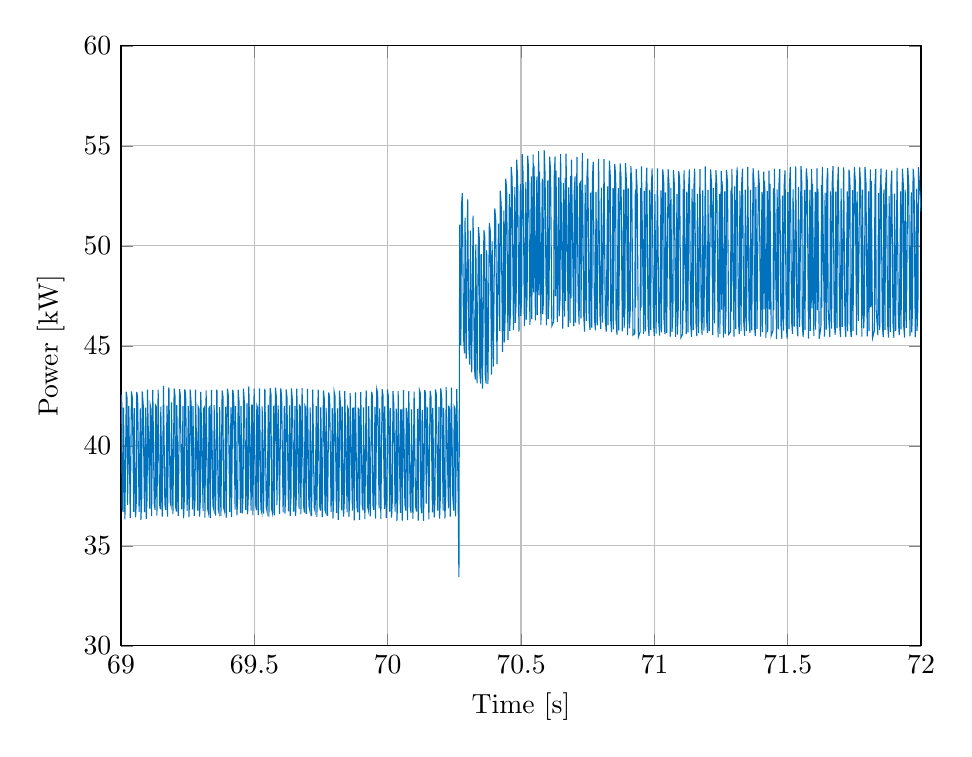
\begin{tikzpicture}

\begin{axis}[%
width=4.0in,
height=3.0in,
at={(0.758in,0.481in)},
scale only axis,
xmin=69,
xmax=72,
xlabel={Time [s]},
xmajorgrids,
ymin=30,
ymax=60,
ylabel={Power [kW]},
ymajorgrids,
axis background/.style={fill=white}
]
\addplot [color=mycolor1,solid,forget plot]
  table[row sep=crcr]{%
69	42.0960090642869\\
69.00238	42.5559127479842\\
69.00448	36.9304035360587\\
69.00788	36.6986566116855\\
69.0092	41.9040380689165\\
69.01452	36.3199030238924\\
69.0198	42.7008963276288\\
69.02228	42.4192813188401\\
69.02452	37.0509363491857\\
69.02918	41.9996463688265\\
69.03454	36.3947483400785\\
69.03458	36.4410586652751\\
69.03918	42.7221469649957\\
69.04236	42.3933520014313\\
69.04792	36.6963423109946\\
69.0499	41.8899368936894\\
69.05454	36.4234595826002\\
69.05786	37.3699294333512\\
69.05916	42.6899957342084\\
69.06226	42.4038924677669\\
69.06788	36.6999047397127\\
69.07238	41.8721813488837\\
69.07456	36.2972837091461\\
69.0778	37.4358016851034\\
69.07922	42.7229193761768\\
69.0831	42.1095546802261\\
69.0879	36.6864335616395\\
69.09234	41.9090754786125\\
69.09454	36.3530078466834\\
69.09788	37.4736333563494\\
69.09924	42.803456752\\
69.10788	36.8654118284957\\
69.1092	42.053927176649\\
69.11236	41.8526943259543\\
69.1146	36.487117478319\\
69.11916	42.8016329754773\\
69.12444	37.1177209561857\\
69.12794	36.79171310045\\
69.12988	42.0205814942576\\
69.1324	41.954159768411\\
69.13454	36.5077477883357\\
69.13922	42.8079391245626\\
69.14452	37.0621687492813\\
69.14788	36.8206470621655\\
69.14924	41.9535676146947\\
69.15454	36.4610679948756\\
69.159	42.6757066554406\\
69.1592	42.9818657293557\\
69.16448	37.0721743774901\\
69.16792	36.786152688155\\
69.1724	42.0061495743427\\
69.17454	36.4569230249899\\
69.1792	42.915073892547\\
69.17978	42.8051384911361\\
69.18446	37.1797525446474\\
69.18794	36.9837290386078\\
69.1892	42.1755218118723\\
69.19458	36.5808635386711\\
69.1992	42.8726922139985\\
69.20236	42.5029991764865\\
69.2045	36.9679436405511\\
69.2079	36.7118718139959\\
69.20916	42.0321879179646\\
69.21454	36.4941907596754\\
69.21976	42.8314160043567\\
69.22228	42.5236552886485\\
69.22794	36.8211016657531\\
69.23232	41.9880176153725\\
69.23456	36.3773625124651\\
69.23784	37.5166323154776\\
69.23916	42.8174871562231\\
69.24232	42.590353934823\\
69.24788	36.7503466947837\\
69.25226	41.9948603146254\\
69.25454	36.4288644289047\\
69.25782	37.5208282942826\\
69.25912	42.8203444510937\\
69.26304	42.110040536459\\
69.26786	36.824783134485\\
69.26978	41.9860289022677\\
69.27454	36.4985082200892\\
69.2778	37.388844183683\\
69.27912	42.8050592828384\\
69.2879	36.7534873638932\\
69.28916	41.9644014044407\\
69.29228	41.8569769949865\\
69.2945	36.4587110791705\\
69.29784	37.4018825436509\\
69.29912	42.7001597566365\\
69.30786	36.7372144598477\\
69.30912	41.8394833021144\\
69.31232	41.9174742451826\\
69.31446	36.407544666765\\
69.31914	42.77189820798\\
69.32448	36.8780068976299\\
69.32786	36.6577634656352\\
69.3298	41.8818526132918\\
69.33238	41.9412082546322\\
69.33452	36.3830499324044\\
69.3391	42.7921672914878\\
69.34446	37.0097091863565\\
69.34788	36.8212195523597\\
69.34918	42.0316253352224\\
69.35446	36.5085142398206\\
69.35914	42.8028840999977\\
69.35978	42.7308984749884\\
69.36446	36.8317367049195\\
69.36784	36.6425410625091\\
69.36986	41.93765235963\\
69.37454	36.4997869016355\\
69.37918	42.7663234961048\\
69.3823	42.4607232735905\\
69.38446	36.9269220451554\\
69.3879	36.7404906274645\\
69.39238	41.9457678173549\\
69.39452	36.4035279290206\\
69.39916	42.8613109897251\\
69.40236	42.5040022099868\\
69.40782	36.6954435348295\\
69.41236	41.9242553436566\\
69.41452	36.4317646157955\\
69.41476	37.0588116662464\\
69.41918	42.8055489910929\\
69.42226	42.4343695662523\\
69.42788	36.8109381920963\\
69.42922	41.9893380110246\\
69.43456	36.5288328574307\\
69.4378	37.4111151810318\\
69.43914	42.8096294189846\\
69.4424	42.2350981400335\\
69.44794	36.6461690103002\\
69.4499	41.979658643863\\
69.45452	36.6182238286659\\
69.4578	37.5080650981595\\
69.45918	42.8559135535829\\
69.46314	42.0411276929031\\
69.46788	36.7851028227498\\
69.47226	42.118916774762\\
69.47454	36.5688613736583\\
69.4778	37.6250868880573\\
69.47918	42.9697407046519\\
69.48794	36.7646662185471\\
69.48986	42.0351962137481\\
69.49236	42.0361810071846\\
69.49454	36.5193737098206\\
69.49916	42.8620786088031\\
69.50446	37.0578649575612\\
69.50788	36.7793626852272\\
69.50922	42.0225589214941\\
69.51238	41.8944825193229\\
69.5145	36.5327212654563\\
69.51912	42.8688581051802\\
69.52444	36.8543179818252\\
69.5279	36.6547344981785\\
69.52916	41.9774191997382\\
69.53456	36.6068834346194\\
69.53916	42.7941129209847\\
69.53974	42.7837982394699\\
69.54452	36.9256417413792\\
69.5479	36.7050533784797\\
69.55232	42.0417907518976\\
69.55454	36.4637929455961\\
69.55914	42.895415486223\\
69.56236	42.5572723675891\\
69.5645	36.8584055010284\\
69.56784	36.6438912346442\\
69.57236	41.9988491640251\\
69.57452	36.5215951636116\\
69.57912	42.9030254298698\\
69.58226	42.4721688147962\\
69.58448	37.034132909233\\
69.5892	42.0190249373194\\
69.59446	36.6333491906225\\
69.59452	36.5982302821719\\
69.59914	42.8737160126058\\
69.60234	42.4063261330556\\
69.60786	36.6724513371134\\
69.61236	41.9903464607732\\
69.61454	36.6102046278257\\
69.61774	37.5731619716849\\
69.61918	42.8226545773196\\
69.62226	42.4460644797842\\
69.62786	36.7232732693329\\
69.63226	42.0212667813456\\
69.63452	36.4991020600841\\
69.6378	37.5741224595183\\
69.63908	42.8657702982625\\
69.64308	42.1533547120755\\
69.64784	36.7065393692507\\
69.65226	41.9918094850021\\
69.6545	36.4806024986324\\
69.65776	37.5760328326756\\
69.65916	42.8587972534398\\
69.6678	36.8337109058741\\
69.66914	42.0196817592662\\
69.67226	41.9535243730622\\
69.67452	36.5865079747009\\
69.67908	42.8851210679419\\
69.68434	37.0164445499283\\
69.68784	36.6608366574602\\
69.68984	41.9880457954753\\
69.69236	41.8906351024035\\
69.69446	36.6019866596949\\
69.69912	42.8403754795681\\
69.70444	37.0022050329855\\
69.70786	36.7768392610297\\
69.70914	41.9176533135105\\
69.71448	36.4810131862259\\
69.7189	42.4050407810376\\
69.71908	42.8068381370481\\
69.72444	36.9350586779022\\
69.72788	36.7373228123708\\
69.73222	41.9812202700803\\
69.73452	36.4482173644258\\
69.73914	42.8121520067398\\
69.73972	42.7135639428442\\
69.74444	37.0044698724979\\
69.74782	36.7570272666854\\
69.74916	41.9263731958314\\
69.75448	36.4305931426707\\
69.75908	42.7642749899312\\
69.7623	42.329544517957\\
69.76446	36.8039268639819\\
69.76782	36.6717828391125\\
69.76916	41.8965328448592\\
69.7745	36.4979571222339\\
69.77912	42.6639264703874\\
69.78226	42.3699744944883\\
69.78786	36.6961571853764\\
69.7923	41.8776065753919\\
69.79452	36.364257480237\\
69.79778	37.4123091368669\\
69.79914	42.714239762884\\
69.80234	42.5033927383611\\
69.80782	36.6428529438385\\
69.81224	41.8693333666181\\
69.8145	36.303175864263\\
69.81774	37.4123313761866\\
69.81916	42.7569423768142\\
69.82302	42.0705679621064\\
69.82782	36.7724567682369\\
69.82976	41.9534202542857\\
69.83448	36.455942944107\\
69.83772	37.3257198163572\\
69.8391	42.7341242785117\\
69.84786	36.6695134425217\\
69.84974	41.9192503473183\\
69.85228	41.8234992149201\\
69.85448	36.4379300577773\\
69.85778	37.3533376711531\\
69.85916	42.6520996667939\\
69.8678	36.7561284869509\\
69.86914	41.8756984544379\\
69.8723	41.8753398842983\\
69.87448	36.2689492537303\\
69.87906	42.673723185013\\
69.88444	36.9482302550381\\
69.88782	36.6794774124858\\
69.88978	41.8730640727767\\
69.89226	41.8227102790494\\
69.89446	36.299687826756\\
69.8991	42.6791835505121\\
69.90444	37.0054999908332\\
69.90782	36.7685965083308\\
69.90916	41.9177155668194\\
69.91446	36.3318083734199\\
69.9191	42.7692211022521\\
69.91974	42.6682597928314\\
69.92444	36.9583777985286\\
69.92782	36.7610511912757\\
69.92916	41.9777344976742\\
69.93444	36.4694139772641\\
69.93972	42.7071721658007\\
69.94226	42.5203160639268\\
69.9444	37.040660311027\\
69.94782	36.8009511791569\\
69.95236	41.9439478633753\\
69.95452	36.3533483033263\\
69.95914	42.8359017849269\\
69.96234	42.6233830320923\\
69.96776	36.8665328345388\\
69.96984	41.8724544675611\\
69.97448	36.3520956009231\\
69.97468	36.8060974517473\\
69.97912	42.8304582964292\\
69.98228	42.5371843267494\\
69.98782	36.8442465988498\\
69.9891	41.9757908000066\\
69.99448	36.3964010888729\\
69.9978	37.4176116882202\\
69.99908	42.8177555747184\\
70.00232	42.484527445938\\
70.00786	36.7113305992732\\
70.00984	41.8856763746872\\
70.0145	36.4156829239612\\
70.01782	37.3991650847187\\
70.0197	42.7336589990408\\
70.02314	42.0755950250889\\
70.02782	36.7151396052684\\
70.03228	41.8643233127954\\
70.03452	36.2389573116088\\
70.03778	37.3723718319427\\
70.03912	42.7285120506424\\
70.04788	36.6496405318085\\
70.04914	41.793721201515\\
70.0523	41.7963466234005\\
70.05452	36.2534007846297\\
70.05918	42.7783813058802\\
70.06444	37.0672784807627\\
70.0679	36.765071488122\\
70.06918	41.901030034585\\
70.07228	41.6752178202025\\
70.07454	36.2889092215104\\
70.07918	42.7296110069536\\
70.08444	36.9184431859163\\
70.08788	36.6537777013455\\
70.08922	41.8198808324584\\
70.0945	36.3479600766345\\
70.0991	42.7096092634951\\
70.10446	36.9846087586051\\
70.10782	36.7112646769021\\
70.1123	41.8483568369744\\
70.11456	36.2573770911153\\
70.11914	42.7770127146621\\
70.1223	42.6296559544271\\
70.12448	36.9821079937539\\
70.12788	36.6300343687272\\
70.12982	41.7976287282342\\
70.13454	36.2420937164587\\
70.13916	42.7871454197887\\
70.1423	42.533514984814\\
70.14442	37.1082496000103\\
70.14912	41.9265248766925\\
70.1544	36.4299458695279\\
70.15444	36.3175826285389\\
70.1591	42.75221349622\\
70.16232	42.4511792064021\\
70.16786	36.6731747832976\\
70.16914	41.8915582455588\\
70.17448	36.4204421342659\\
70.17776	37.4405341217313\\
70.17916	42.8228488278424\\
70.18226	42.5801851776344\\
70.18784	36.7604632167825\\
70.1923	41.9403646247269\\
70.19454	36.3555067638187\\
70.19776	37.5714972191957\\
70.1991	42.8752468482219\\
70.20312	42.292661758565\\
70.20788	36.7628987651489\\
70.2098	41.900182952876\\
70.21446	36.3630673153674\\
70.21776	37.5400264214233\\
70.21914	42.9327582937706\\
70.2278	36.8665092742814\\
70.22916	42.0076093979571\\
70.23224	41.7879450409198\\
70.23446	36.4638425430387\\
70.2391	42.9061895585622\\
70.24426	37.3739368537502\\
70.24784	36.756891812381\\
70.24914	41.9703978986432\\
70.25236	41.8643394481613\\
70.25452	36.4757961823336\\
70.25914	42.8340255801467\\
70.26444	37.0901425588157\\
70.26712	33.4333518715314\\
70.2701	51.0612878172907\\
70.27442	45.0270296557091\\
70.27682	52.0299781725829\\
70.27996	52.6370796498976\\
70.28452	45.4213424162415\\
70.28794	44.6237789459264\\
70.29016	51.415011874031\\
70.29466	44.3580493103096\\
70.29936	51.5584043448115\\
70.29996	52.3206350845798\\
70.30472	44.8785884544262\\
70.30814	44.041840018107\\
70.31022	50.7605625085435\\
70.31492	43.6763221523153\\
70.32018	51.5075105455175\\
70.32032	51.3829253849544\\
70.32496	44.0128361249953\\
70.32838	43.3254468917184\\
70.3305	50.0694149513089\\
70.33518	43.1232268968911\\
70.34042	50.9410201240271\\
70.34392	50.3253953211744\\
70.34524	43.6762499398367\\
70.34868	43.1052248172896\\
70.35084	49.5799595597726\\
70.3555	42.8578169457409\\
70.36076	50.7819782570496\\
70.36432	50.4067160630674\\
70.36556	43.606190474468\\
70.3691	43.1134425602216\\
70.37114	49.7741295280009\\
70.37582	43.0844331900038\\
70.38116	51.1493496309611\\
70.38466	50.7323737407894\\
70.38942	43.6363414286325\\
70.38948	43.5610609514674\\
70.39156	50.2168431668401\\
70.39634	43.9556051350353\\
70.40168	51.8677379148232\\
70.40512	51.2971696856992\\
70.4099	44.0849771804608\\
70.41016	44.6863176272748\\
70.41538	51.1031476588399\\
70.42012	45.7436161754844\\
70.4221	52.7617468270531\\
70.4256	52.051468648218\\
70.43046	44.6920663529853\\
70.43584	51.7687343198908\\
70.43722	45.1753983882474\\
70.4406	46.4681780780348\\
70.44264	53.3524229498904\\
70.44614	52.8463425475193\\
70.45096	45.297907407443\\
70.45644	52.5797504900231\\
70.4578	45.7513244890023\\
70.4612	47.0941907068898\\
70.46318	53.9448211026162\\
70.46664	53.3498162768413\\
70.4715	45.7905099944217\\
70.47696	52.9290799038313\\
70.4783	46.1417471975033\\
70.48176	47.1715338491421\\
70.48376	54.3076377929939\\
70.48732	53.3087210867324\\
70.49214	45.7036512918599\\
70.49754	53.0939652307264\\
70.49894	46.4921270408411\\
70.50234	47.3220693284716\\
70.50434	54.5801847824257\\
70.50784	53.5357680014059\\
70.51268	45.9817782959345\\
70.51814	53.1780776438423\\
70.51954	46.3042209255278\\
70.52296	47.557876400469\\
70.52496	54.5104504956446\\
70.52842	53.8084588406305\\
70.53334	46.0505475641449\\
70.53878	53.474135757836\\
70.54016	46.3291178845373\\
70.54554	54.5761580493906\\
70.54702	47.6685151766476\\
70.54906	53.9946394665389\\
70.55394	46.2765422060897\\
70.5593	53.4605161624306\\
70.56076	46.5471472561103\\
70.56616	54.7370809573415\\
70.5676	47.5242556654587\\
70.56964	53.7100069786024\\
70.57452	46.048206073811\\
70.5799	53.3642183835991\\
70.58136	46.5870739632439\\
70.58474	47.3738460134918\\
70.58676	54.7811459105041\\
70.5902	53.5741387458698\\
70.59512	46.0162184950858\\
70.60044	53.2689257670258\\
70.60192	46.3407001039976\\
70.60526	47.4838924597703\\
70.6073	54.4591865949604\\
70.61076	53.728757906489\\
70.61564	45.995902235353\\
70.62248	46.2101188146408\\
70.62442	53.4178719597936\\
70.62776	54.4665928610968\\
70.6293	47.4830182607215\\
70.63138	53.7553171972382\\
70.63614	46.1953934157764\\
70.64156	53.4171777168288\\
70.643	46.4713864214292\\
70.64636	47.3768712027847\\
70.64832	54.6002975744565\\
70.65666	45.8569787963197\\
70.65884	53.1335981567439\\
70.66344	46.458594163468\\
70.6654	53.3697027612792\\
70.66686	47.2460673257569\\
70.66878	54.6142378771633\\
70.67714	45.9288887794314\\
70.67916	52.9213374657093\\
70.68394	46.1384706541846\\
70.68598	53.4896855512499\\
70.6873	47.3767854949597\\
70.68922	54.3032857271693\\
70.69754	45.9856948182314\\
70.69968	52.7660264259117\\
70.7029	53.4712901047816\\
70.70436	46.1638417997717\\
70.7097	54.4434781959212\\
70.7143	47.2733834995909\\
70.71794	46.0634317883033\\
70.71994	53.0916339012504\\
70.72332	53.183397416083\\
70.72472	46.3679717648648\\
70.73006	54.6456812078542\\
70.73486	46.6017512488447\\
70.73832	45.7060870112994\\
70.74036	53.059097481874\\
70.74506	46.2518721969053\\
70.7471	53.3391132704582\\
70.75038	54.361081973192\\
70.75524	46.3817388956859\\
70.75864	45.7970685573912\\
70.76066	52.6545703831312\\
70.7654	45.9109058804537\\
70.76742	53.2095452892685\\
70.77068	54.1948604126283\\
70.77548	46.3621983123932\\
70.77896	45.7759002862416\\
70.78094	52.6828063269633\\
70.78568	46.0245537717798\\
70.79034	53.7257682896201\\
70.79088	54.3422643429994\\
70.79576	46.578120088384\\
70.79922	45.8312285475219\\
70.80118	52.9070097043879\\
70.80596	46.163135245419\\
70.81108	54.1259960074531\\
70.81118	54.3399655847597\\
70.81594	46.370086974186\\
70.81938	45.7072377065637\\
70.82474	52.9720049111994\\
70.8261	46.0348100332574\\
70.83136	54.2607443313268\\
70.83476	53.4765411760567\\
70.83612	46.3409434972265\\
70.83962	45.6858143360648\\
70.84484	52.8878387832955\\
70.8463	45.821731262282\\
70.8515	54.0868203392586\\
70.85496	53.4425537299104\\
70.85622	46.2893706910563\\
70.85974	45.5612079733088\\
70.86498	52.8882747486843\\
70.86644	45.7693331176533\\
70.8716	54.1204405474887\\
70.87504	53.4006889979986\\
70.8798	45.7267285306345\\
70.88506	52.8151350209591\\
70.88646	45.8803454051915\\
70.88976	46.8893219738248\\
70.89172	54.1289831019751\\
70.89522	53.2125391039367\\
70.89984	45.5363517421172\\
70.902	52.8752164079188\\
70.90658	45.8760425090686\\
70.90982	46.8630037113443\\
70.91176	53.9865188452069\\
70.91512	53.1723407594623\\
70.9199	45.5343328152526\\
70.9266	45.6081575584656\\
70.9286	52.8111042707701\\
70.92984	46.9075678156745\\
70.93178	53.8425325440476\\
70.9355	52.8444890512657\\
70.93996	45.4385480618212\\
70.94656	45.6980239149082\\
70.94872	52.8882699966355\\
70.94984	46.9055728687006\\
70.95174	53.9704814822403\\
70.95994	45.6019429247602\\
70.96206	52.7520019525097\\
70.96656	45.7251724898296\\
70.96866	52.8450416537913\\
70.97172	53.9029444009135\\
70.97648	46.0945817472229\\
70.97988	45.4944010977029\\
70.98204	52.7986397507548\\
70.9865	45.7987218283703\\
70.98858	52.8380118482897\\
70.99168	53.8662395758284\\
70.99648	46.1781583892232\\
70.99986	45.4871108204855\\
71.00196	52.5812407753444\\
71.00652	45.6119390277517\\
71.01154	53.5642499406528\\
71.01166	53.8755023989569\\
71.01638	46.1930321984351\\
71.01978	45.5102786457739\\
71.02506	52.7751795374079\\
71.02644	45.666844549586\\
71.03162	53.8204830261127\\
71.035	53.2166341297505\\
71.03636	46.2295441526076\\
71.03976	45.5867395357371\\
71.04184	52.6738603948888\\
71.04638	45.650931677116\\
71.0516	53.8317166394311\\
71.05504	53.0551145567429\\
71.05966	45.4552626139033\\
71.06184	52.8988746667906\\
71.06632	45.702507006692\\
71.06958	46.6774869894146\\
71.0715	53.7784324843029\\
71.07494	53.0653782256745\\
71.07964	45.4515267155651\\
71.08484	52.5988589124266\\
71.08626	45.5598736672088\\
71.08948	46.7900686135001\\
71.09136	53.7262798437442\\
71.09486	53.3126747061282\\
71.09956	45.4126530847545\\
71.10618	45.5812691548811\\
71.10826	52.8313134363347\\
71.10942	46.7704094006248\\
71.1114	53.775489125655\\
71.11942	45.5805132050611\\
71.12148	52.7039878462102\\
71.1261	45.6762864177441\\
71.12826	52.7666402185948\\
71.13126	53.8183865067846\\
71.13594	46.1676705503499\\
71.13934	45.4510834156985\\
71.14148	52.8505507288321\\
71.14598	45.7880589007258\\
71.14812	52.8728054102785\\
71.15114	53.8554514106023\\
71.1559	46.1890533353317\\
71.15928	45.4875206927114\\
71.16144	52.6010246977267\\
71.16592	45.6383539910224\\
71.17054	53.1326230870118\\
71.17112	53.8298457471931\\
71.1758	46.2639093163582\\
71.1792	45.5457551969846\\
71.18138	52.7703770438821\\
71.18584	45.7619325017938\\
71.19104	53.9710059911579\\
71.19126	53.6005547822995\\
71.19568	46.328592518036\\
71.19916	45.6422609399174\\
71.2011	52.7916659502918\\
71.20574	45.7495074352876\\
71.21092	53.8242368660776\\
71.21434	53.1105267545364\\
71.21892	45.8014730331351\\
71.21906	45.5375154027807\\
71.22122	52.8863051217464\\
71.22584	46.1162649437828\\
71.23082	53.7847107447256\\
71.23424	52.9998205496609\\
71.23902	45.4215595723371\\
71.24416	52.5778840397923\\
71.24564	45.5963351028877\\
71.25076	53.7523653072162\\
71.25226	46.8153623547406\\
71.25428	53.228351465265\\
71.25888	45.4089775335227\\
71.26416	52.7226505906436\\
71.26552	45.5804281443879\\
71.26878	46.8440569700461\\
71.27068	53.7983085410215\\
71.27422	53.1670421717814\\
71.27878	45.5776362640795\\
71.28542	45.697043742227\\
71.2876	52.7739070520813\\
71.28872	46.7123560619483\\
71.29066	53.8404692782426\\
71.2987	45.455341253429\\
71.30082	52.967622311168\\
71.30534	45.8341020324545\\
71.3075	53.0162246513311\\
71.31054	53.9218924139003\\
71.31522	46.2004990300383\\
71.31864	45.5837536934881\\
71.32078	52.7494812496192\\
71.3253	45.7367725811661\\
71.32728	53.0100687352494\\
71.33046	53.8583271865866\\
71.33514	46.1856147666826\\
71.33854	45.4951831614787\\
71.34076	52.809506645643\\
71.3452	45.739567552735\\
71.35026	53.74352230674\\
71.35034	53.9433276684657\\
71.35506	46.236207372945\\
71.35848	45.653496394306\\
71.36062	52.7951805276131\\
71.36512	45.7759925223722\\
71.37026	53.8794699046798\\
71.37376	53.1044121280087\\
71.37498	46.0806476844957\\
71.37844	45.4868144744202\\
71.38058	52.9282167531453\\
71.38502	45.8503500080722\\
71.39028	53.7718272174376\\
71.39366	53.0253042356665\\
71.39838	45.4594464350904\\
71.40354	52.6916534151757\\
71.40502	45.6852258456259\\
71.4102	53.7071814641592\\
71.4116	46.8211955279325\\
71.41358	53.2477445173588\\
71.41832	45.3907465967294\\
71.4235	52.7373899113007\\
71.42494	45.6889670158353\\
71.43008	53.7636343634088\\
71.43158	46.8197989979884\\
71.43352	53.1012451632762\\
71.43824	45.5120156820241\\
71.4449	45.7741150182542\\
71.44686	52.8660004480151\\
71.44816	46.788708962806\\
71.45008	53.8548757857459\\
71.45822	45.3392168913569\\
71.46038	52.8192970747851\\
71.46482	45.8215205009855\\
71.46696	52.9485101794179\\
71.47004	53.8307051121251\\
71.47468	46.0800369319881\\
71.47818	45.3470706526821\\
71.48038	52.5090702706056\\
71.48484	45.7550091254727\\
71.48692	53.011094034409\\
71.49004	53.7751845303762\\
71.49476	46.0171126873648\\
71.4981	45.345935350152\\
71.50032	52.6876271171174\\
71.50478	45.8388496800331\\
71.50694	53.0939826428947\\
71.50996	53.9490689864845\\
71.51466	46.2266381174789\\
71.5181	45.598964319369\\
71.52022	52.8251470352419\\
71.5248	45.9630681901844\\
71.52994	53.975312020931\\
71.52998	53.9192777078161\\
71.53464	46.0658678056462\\
71.5381	45.4759350071745\\
71.54024	52.9278236844977\\
71.54476	45.9469327005668\\
71.54998	53.9781367845431\\
71.55334	53.0216023359351\\
71.55464	46.0672247166272\\
71.55806	45.4302100667347\\
71.56332	52.7960673500643\\
71.5647	45.7884692867009\\
71.5699	53.8735089682672\\
71.57342	53.2626210893572\\
71.57808	45.3630081685931\\
71.58328	52.7973478406942\\
71.58472	45.7446393374658\\
71.5899	53.85229132014\\
71.5914	46.8677891739702\\
71.59332	53.0964144548605\\
71.59808	45.4913139733374\\
71.6033	52.6933883883415\\
71.60474	45.8076804813001\\
71.60994	53.8726274516012\\
71.61144	46.7863236137181\\
71.61334	52.8617153136903\\
71.61806	45.3502748719974\\
71.62468	45.9635046382304\\
71.62668	53.0382351511764\\
71.628	46.9089211281453\\
71.6299	53.9494289280146\\
71.63804	45.461042109999\\
71.6402	52.6431118216925\\
71.64474	45.8141150403477\\
71.6468	53.1759775123072\\
71.64996	53.883022460981\\
71.6514	46.8879095506741\\
71.65804	45.4463659609614\\
71.66018	52.7264287046177\\
71.6647	45.8599489824402\\
71.66692	53.1242565937357\\
71.66998	53.979935575924\\
71.67466	46.1881184604331\\
71.6781	45.55271791248\\
71.68014	52.7041392725163\\
71.68468	45.8762577926624\\
71.6869	52.9409578377688\\
71.68994	53.9523136969509\\
71.69466	46.0751005557795\\
71.6981	45.4371906940874\\
71.70028	52.8665951301647\\
71.70474	45.9454504243325\\
71.70942	53.1604039981791\\
71.70992	53.9223473031121\\
71.7147	46.0774081679726\\
71.71806	45.4407000625245\\
71.72336	52.7221376039639\\
71.72476	45.7302012615513\\
71.73004	53.8099730197797\\
71.7334	53.2686401201852\\
71.73472	46.0269367833876\\
71.73812	45.4335099851671\\
71.74346	52.7873092892084\\
71.7448	45.7293354849006\\
71.75	53.9497010490111\\
71.75348	53.231161124839\\
71.7581	45.62922828975\\
71.75814	45.5335702763121\\
71.76026	52.7145111114315\\
71.765	46.2451881997123\\
71.77002	53.9196814621306\\
71.77342	53.0470056053912\\
71.77818	45.4631350951541\\
71.78036	52.8110711129915\\
71.78488	45.8701628601327\\
71.78818	46.8923014426777\\
71.79008	53.9322144290508\\
71.79348	53.1432967423413\\
71.79818	45.4671469355143\\
71.80346	52.7225432075655\\
71.80488	45.7318839286489\\
71.81008	53.8194148640969\\
71.81162	46.9350148922799\\
71.81358	53.2514693485467\\
71.81824	45.391950731599\\
71.82492	45.7622832016656\\
71.82712	52.9400956973315\\
71.8301	53.8441171992288\\
71.83156	46.8356171323209\\
71.8383	45.526069851479\\
71.8404	52.6324168520036\\
71.84496	45.7895375075205\\
71.84706	52.8336770337942\\
71.85014	53.8649545795265\\
71.85484	46.0582027818685\\
71.85828	45.4302086542731\\
71.86046	52.8107412541967\\
71.86496	45.8001400185275\\
71.86696	52.874324180956\\
71.8702	53.8047196522671\\
71.87492	46.0321149627677\\
71.87832	45.4081487450516\\
71.88038	52.4780615101239\\
71.88494	45.6927567221298\\
71.8871	52.938330651442\\
71.89022	53.7600860257251\\
71.89496	46.1237513000333\\
71.89834	45.3899405502807\\
71.9005	52.6137415783747\\
71.90496	45.7476822300895\\
71.91016	53.8464769291072\\
71.9102	53.8929121342285\\
71.91496	46.2344067936436\\
71.91834	45.5359331500602\\
71.92362	52.7188728994013\\
71.925	45.8253860071405\\
71.93022	53.8543965895169\\
71.93376	52.9999268539752\\
71.93496	46.0157395135321\\
71.93838	45.4109499564233\\
71.94054	52.8117236847835\\
71.94502	45.8907996647965\\
71.9503	53.8903208988447\\
71.95372	53.113645385727\\
71.9584	45.4687743282712\\
71.96366	52.6676916031822\\
71.96506	45.6776161737613\\
71.96834	46.8777312225649\\
71.97026	53.8569326329298\\
71.97378	53.3118080674071\\
71.97844	45.4383063290145\\
71.98362	52.8455554249023\\
71.98502	45.7419538949208\\
71.98834	46.9331212412499\\
71.9903	53.9297977549192\\
72.00002	51.7077566657693\\
};
\end{axis}
\end{tikzpicture}%
\caption{Power step from 40 to 50 kW performed on a genset located at DEIF and measured by Hioki oscilliscope at 50 kHz sampling rate.}
\label{fig:gensetPowermeas}
\end{figure}

\begin{figure}[H]
\centering
% This file was created by matlab2tikz.
%
%The latest updates can be retrieved from
%  http://www.mathworks.com/matlabcentral/fileexchange/22022-matlab2tikz-matlab2tikz
%where you can also make suggestions and rate matlab2tikz.
%
\definecolor{mycolor1}{rgb}{0.00000,0.44700,0.74100}%
%
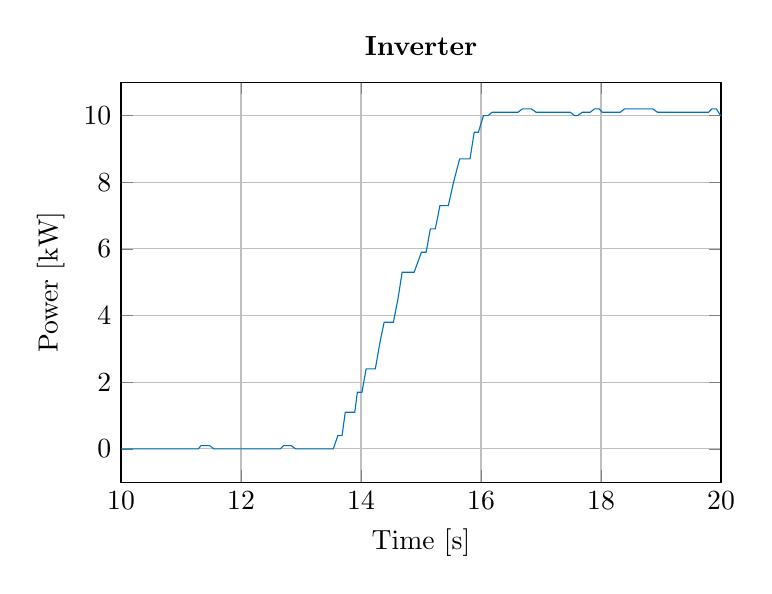
\begin{tikzpicture}

\begin{axis}[%
width=3.0in,
height=2.0in,
at={(0.758in,0.481in)},
scale only axis,
xmin=10,
xmax=20,
xlabel={Time [s]},
xmajorgrids,
ymin=-1,
ymax=11,
ylabel={Power [kW]},
ymajorgrids,
axis background/.style={fill=white},
title style={font=\bfseries},
title={Inverter}
]
\addplot [color=mycolor1,solid,forget plot]
  table[row sep=crcr]{%
9.997	0\\
10.067	0\\
10.138	0\\
10.218	0\\
10.278	0\\
10.348	0\\
10.431	0\\
10.508	0\\
10.578	0\\
10.633	0\\
10.708	0\\
10.778	0\\
10.848	0\\
10.932	0\\
10.998	0\\
11.088	0\\
11.178	0\\
11.198	0\\
11.288	0\\
11.332	0.1\\
11.408	0.1\\
11.478	0.1\\
11.548	0\\
11.632	0\\
11.708	0\\
11.778	0\\
11.831	0\\
11.909	0\\
11.979	0\\
12.049	0\\
12.131	0\\
12.209	0\\
12.279	0\\
12.332	0\\
12.409	0\\
12.48	0\\
12.55	0\\
12.651	0\\
12.71	0.1\\
12.751	0.1\\
12.834	0.1\\
12.912	0\\
12.992	0\\
13.036	0\\
13.112	0\\
13.193	0\\
13.236	0\\
13.313	0\\
13.383	0\\
13.454	0\\
13.537	0\\
13.614	0.4\\
13.684	0.4\\
13.737	1.1\\
13.814	1.1\\
13.895	1.1\\
13.939	1.7\\
14.015	1.7\\
14.085	2.4\\
14.155	2.4\\
14.238	2.4\\
14.316	3.2\\
14.385	3.8\\
14.455	3.8\\
14.539	3.8\\
14.616	4.5\\
14.685	5.3\\
14.739	5.3\\
14.816	5.3\\
14.885	5.3\\
15.006	5.9\\
15.015	5.9\\
15.085	5.9\\
15.155	6.6\\
15.238	6.6\\
15.315	7.3\\
15.385	7.3\\
15.455	7.3\\
15.542	8\\
15.643	8.7\\
15.686	8.7\\
15.739	8.7\\
15.816	8.7\\
15.886	9.5\\
15.956	9.5\\
16.041	10\\
16.116	10\\
16.186	10.1\\
16.239	10.1\\
16.316	10.1\\
16.386	10.1\\
16.457	10.1\\
16.54	10.1\\
16.617	10.1\\
16.687	10.2\\
16.757	10.2\\
16.842	10.2\\
16.917	10.1\\
16.987	10.1\\
17.057	10.1\\
17.145	10.1\\
17.187	10.1\\
17.257	10.1\\
17.343	10.1\\
17.418	10.1\\
17.488	10.1\\
17.558	10\\
17.608	10\\
17.689	10.1\\
17.742	10.1\\
17.819	10.1\\
17.889	10.2\\
17.969	10.2\\
18.019	10.1\\
18.089	10.1\\
18.159	10.1\\
18.242	10.1\\
18.32	10.1\\
18.39	10.2\\
18.46	10.2\\
18.543	10.2\\
18.69	10.2\\
18.72	10.2\\
18.791	10.2\\
18.861	10.2\\
18.943	10.1\\
19.021	10.1\\
19.081	10.1\\
19.152	10.1\\
19.232	10.1\\
19.292	10.1\\
19.361	10.1\\
19.444	10.1\\
19.522	10.1\\
19.592	10.1\\
19.644	10.1\\
19.722	10.1\\
19.792	10.1\\
19.846	10.2\\
19.923	10.2\\
19.993	10\\
20.064	10\\
};
\end{axis}
\end{tikzpicture}%
\caption{Power step from 0 to 10 kW performed on a SMA STP20000 inverter, where measurements is extracted from the inverter via modbus at a sample rate of approximately 14 Hz.}
\label{fig:inverter10kwstep}
\end{figure}


The two measurements show considerable differences concerning the reaction time and the reaction to noise. It can be clearly seen that the inverter is not suitable to be the subject of control due to its slowness. In other words, this slow behaviour makes the inverter incapable of removing sudden disturbances from the output power. As it is illustrated, this is because of the limited rate of power delivery speed of the inverter. 
%The reaction time on the other hand shows that the inverter is not fit to be the subject of control to remove sudden disturbances, due to changes in the load.
The disturbance that can occur and therefore required to be corrected is shown in \figref{fig:gensetPowermeas}. A dip in power appears after the load increases at 70.25 seconds in the graph. The instability arises as the diesel engine can not instantly adjust for the sudden increase in load and the governor needs time to stabilize fuel input. On \figref{fig:4050kwstepfreq} the disturbance in electrical frequency due to a 40 kW to 50 kW step is shown.

\begin{figure}[H]
\centering
% This file was created by matlab2tikz.
%
%The latest updates can be retrieved from
%  http://www.mathworks.com/matlabcentral/fileexchange/22022-matlab2tikz-matlab2tikz
%where you can also make suggestions and rate matlab2tikz.
%
\definecolor{mycolor1}{rgb}{0.00000,0.44700,0.74100}%
%
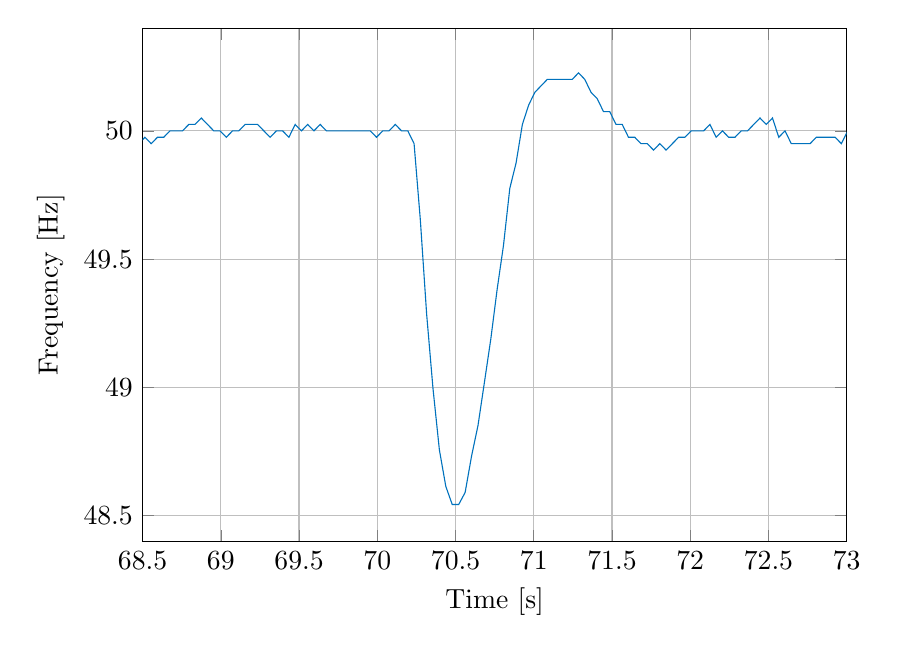
\begin{tikzpicture}

\begin{axis}[%
width=3.521in,
height=2.566in,
at={(0.758in,0.481in)},
scale only axis,
xmin=68.5,
xmax=73,
xlabel={Time [s]},
xmajorgrids,
ymin=48.4,
ymax=50.4,
ylabel={Frequency [Hz]},
ymajorgrids,
axis background/.style={fill=white}
]
\addplot [color=mycolor1,solid,forget plot]
  table[row sep=crcr]{%
68.4752	49.950049950044\\
68.51524	49.9750124937551\\
68.55526	49.9500499500618\\
68.5953	49.9750124937374\\
68.63532	49.9750124937551\\
68.67534	50.0000000000099\\
68.71534	49.9999999999922\\
68.75534	50.0000000000099\\
68.79534	50.0250125062355\\
68.83532	50.025012506271\\
68.8753	50.0500500500403\\
68.91526	50.0250125062532\\
68.95524	49.9999999999922\\
68.99524	50.0000000000099\\
69.03524	49.9750124937551\\
69.07526	49.9999999999922\\
69.11526	50.0000000000099\\
69.15526	50.0250125062532\\
69.19524	50.0250125062532\\
69.23522	50.0250125062532\\
69.2752	49.9999999999922\\
69.3152	49.9750124937551\\
69.35522	49.9999999999922\\
69.39522	50.0000000000099\\
69.43522	49.9750124937551\\
69.47524	50.0250125062532\\
69.51522	49.9999999999922\\
69.55522	50.0250125062532\\
69.5952	50.0000000000099\\
69.6352	50.0250125062532\\
69.67518	49.9999999999922\\
69.71518	49.9999999999922\\
69.75518	50.0000000000099\\
69.79518	50.0000000000099\\
69.83518	49.9999999999922\\
69.87518	49.9999999999922\\
69.91518	50.0000000000099\\
69.95518	49.9999999999922\\
69.99518	49.9750124937551\\
70.0352	49.9999999999922\\
70.0752	50.0000000000099\\
70.1152	50.0250125062532\\
70.15518	49.9999999999922\\
70.19518	50.0000000000099\\
70.23518	49.950049950044\\
70.27522	49.6524329692209\\
70.3155	49.2853622474057\\
70.35608	48.9955903968685\\
70.3969	48.7567040468027\\
70.43792	48.6144871171625\\
70.47906	48.5436893203843\\
70.52026	48.543689320401\\
70.56146	48.5908649173897\\
70.60262	48.7329434697912\\
70.64366	48.8519785051221\\
70.6846	49.019607843132\\
70.7254	49.1883915396107\\
70.76606	49.3827160493722\\
70.80656	49.5540138751329\\
70.84692	49.7760079641532\\
70.8871	49.875311720704\\
70.9272	50.0250125062532\\
70.96718	50.1002004008078\\
71.0071	50.1504513540486\\
71.04698	50.1756146512739\\
71.08684	50.2008032128538\\
71.12668	50.2008032128538\\
71.16652	50.2008032128538\\
71.20636	50.2008032128538\\
71.2462	50.2008032128538\\
71.28604	50.2260170768383\\
71.32586	50.2008032128538\\
71.3657	50.1504513540665\\
71.40558	50.1253132832043\\
71.44548	50.0751126690017\\
71.48542	50.0751126690017\\
71.52536	50.0250125062532\\
71.56534	50.0250125062532\\
71.60532	49.9750124937551\\
71.64534	49.9750124937551\\
71.68536	49.950049950044\\
71.7254	49.9500499500618\\
71.76544	49.9251123314889\\
71.8055	49.9500499500618\\
71.84554	49.9251123315066\\
71.8856	49.950049950044\\
71.92564	49.9750124937551\\
71.96566	49.9750124937551\\
72.00568	49.9999999999922\\
72.04568	49.9999999999922\\
72.08568	50.0000000000099\\
72.12568	50.0250125062532\\
72.16566	49.9750124937551\\
72.20568	49.9999999999922\\
72.24568	49.9750124937551\\
72.2857	49.9750124937551\\
72.32572	50.0000000000099\\
72.36572	49.9999999999922\\
72.40572	50.0250125062532\\
72.4457	50.0500500500403\\
72.48566	50.025012506271\\
72.52564	50.0500500500403\\
72.5656	49.9750124937551\\
72.60562	50.0000000000099\\
72.64562	49.950049950044\\
72.68566	49.950049950044\\
72.7257	49.950049950044\\
72.76574	49.9500499500618\\
72.80578	49.9750124937374\\
72.8458	49.9750124937551\\
72.88582	49.9750124937551\\
72.92584	49.9750124937551\\
72.96586	49.950049950044\\
73.0059	50.0000000000099\\
};
\end{axis}
\end{tikzpicture}% 
\caption{Frequency measured on tachometer with Hioki oscilloscope before and after a power step from 40 to 50 kW is performed on a genset located at DEIF.}
\label{fig:4050kwstepfreq}
\end{figure}


Control can be done on the genset by providing a reference and therefore make the output tracking it. According to the system description in \secref{diesel_generator} and according to the previous discussion, there are two parameters which can be controlled on the genset, namely the frequency input of the governor and the voltage to the AVR. To limit the scope of the project, control is focused on correcting the disturbance by doing corrections in the frequency reference to the governor. Furthermore, control is built around the genset in order to provide a kind of extension, an add-on for the inner controllers inside the genset.In \figref{fig:genset_control_approach} this correction approach of the controller to the genset is illustrated.

\begin{figure}[H]
\centering


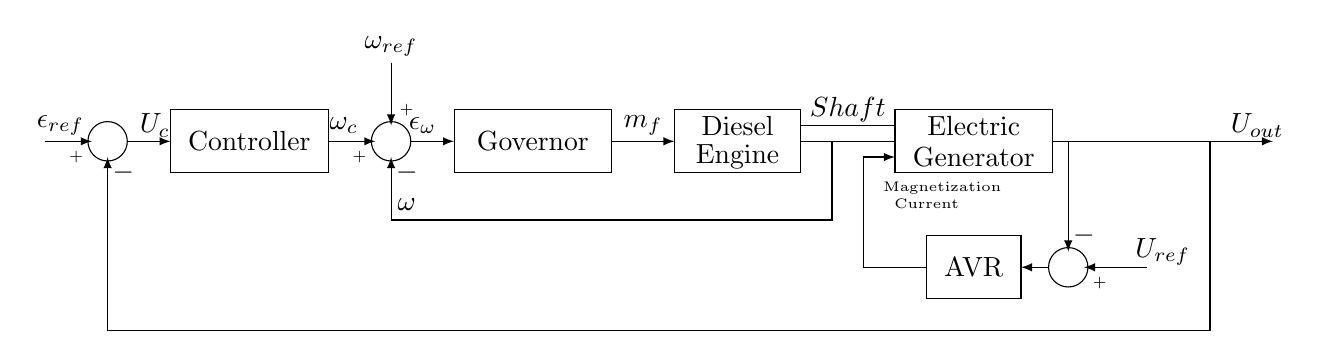
\begin{tikzpicture}

 \node at (2,0.2) {\normalsize{Governor}};
\draw [-latex] (1,0.6) rectangle (3,-0.2);
 \node at (4.6,0.4) {\normalsize{Diesel}};
  \node at (4.6,0) {\normalsize{Engine}};
\draw [-latex] (3.8,0.6) rectangle (5.4,-0.2);
\draw [-latex](3,0.2) -- (3.8,0.2);
\node at (3.4,0.4) {$m_f$};
 \node at (7.6,0.4) {\normalsize{Electric}};
  \node at (7.6,0) {\normalsize{Generator}};
\draw [-latex] (6.6,0.6) rectangle (8.6,-0.2);

\node at (6,0.6) {$Shaft$};
  \node at (7.6,-1.4) {\normalsize{AVR}};
\draw [-latex] (8.8,-1.4) ellipse (0.25 and 0.25);
\draw [-latex] (7,-1) rectangle (8.2,-1.8);
\draw [-latex](7,-1.4) -- (6.2,-1.4) -- (6.2,0) -- (6.6,0);
\node at (9,-1) {$-$};
\draw [-latex](9.8,-1.4) -- (9,-1.4);
\node at (10,-1.2) {$U_{ref}$};
\node at (7.2,-0.4) {\tiny{Magnetization}};
\node at (7,-0.6) {\tiny{Current}};
\node at (11.2,0.4) {$U_{out}$};
\draw [-latex] (0.2,0.2) ellipse (0.25 and 0.25);

\draw [-latex](0.2,1.2) -- (0.2,0.4);
\node at (0.2,1.4) {$\omega_{ref}$};
\draw [-latex](5.8,0.2) -- (5.8,-0.8) -- (0.2,-0.8) -- (0.2,0);
\node at (0.4,-0.6) {$\omega$};
\node at (-1.6,0.2) {\normalsize{Controller}};
\draw [-latex] (-2.6,0.6) rectangle (-0.6,-0.2);
\draw [-latex](-0.6,0.2) -- (0,0.2);
\node at (-0.4,0.4) {$\omega_{c}$};
\draw [-latex] (-3.4,0.2) ellipse (0.25 and 0.25);
\draw [-latex](-3.15,0.2) -- (-2.6,0.2);
\node at (-2.8,0.4) {$U_{c}$};
\draw [-latex](-4.2,0.2) -- (-3.6,0.2);
\node at (-4,0.4) {$\epsilon_{ref}$};
\draw [-latex](10.6,0.2) -- (10.6,-2.2) -- (-3.4,-2.2) -- (-3.4,0);
\node at (-3.2,-0.2) {$-$};
\node at (0.6,0.4) {$\epsilon_{\omega}$};
\draw [-latex](8.8,0.2) -- (8.8,-1.2);
\draw [-latex](8.6,0.2) -- (11.4,0.2);
\draw [-latex](8.55,-1.4) -- (8.2,-1.4);
\draw [thin](5.4,0.2) -- (6.6,0.2);
\draw [thin](5.4,0.4) -- (6.6,0.4);
\draw [thin](0.4,0.2);
\draw [-latex](0.45,0.2) -- (1,0.2);
\node at (-3.8,0) {\tiny{+}};





\node at (9.2,-1.6) {\tiny{+}};
\node at (0.4,-0.2) {$-$};
\node at (0.4,0.6) {\tiny{+}};
\node at (-0.2,0) {\tiny{+}};

\end{tikzpicture} 
%\includegraphics[width=0.6\textwidth]{rapport/billeder/genset_control_approach.png}
\caption{Block diagram illustrating the genset with an addon frequency controller.}
\label{fig:genset_control_approach}
\end{figure}


%This requires the abillity to measure either frequency, Voltage or both on the genset. 
The frequency can be obtained in two ways. Either by making time calculations between zero crossings on one of the three phases of the voltage outputs or by a tachometer. In case of a tachometer, it is required to be installed if it is not already built in the genset. For this reason, voltage measurements are carried out and in the mean time provided to the controller.
When the frequency differs from the reference value after the correction of the governor, in the mean time disturbance will appear in the voltage due to the change in the load, as shown in \figref{fig:4050kwstepvoltage50khz}  

\begin{figure}[H]
\centering
%\includegraphics[width=0.8\textwidth]{rapport/billeder/4050kwstep_rmsvoltage50khz.png}
% This file was created by matlab2tikz.
%
%The latest updates can be retrieved from
%  http://www.mathworks.com/matlabcentral/fileexchange/22022-matlab2tikz-matlab2tikz
%where you can also make suggestions and rate matlab2tikz.
%
\definecolor{mycolor1}{rgb}{0.00000,0.44700,0.74100}%
%
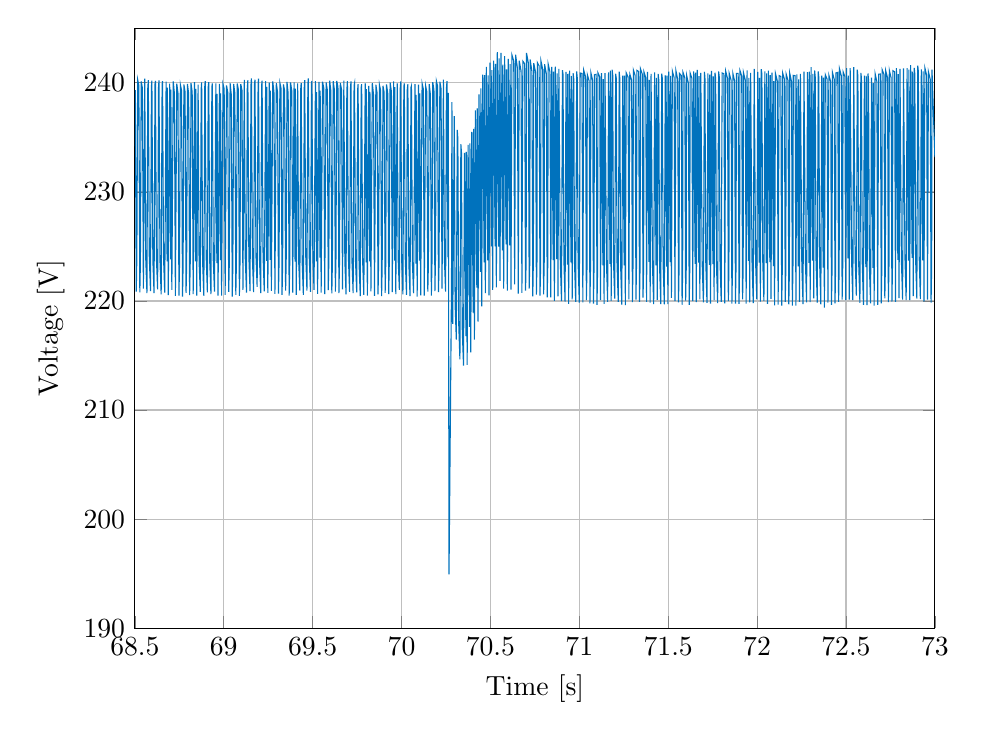
\begin{tikzpicture}

\begin{axis}[%
width=4.0in,
height=3.0in,
at={(0.758in,0.481in)},
scale only axis,
xmin=68.5,
xmax=73,
xlabel={Time [s]},
xmajorgrids,
ymin=190,
ymax=245,
ylabel={Voltage [V]},
ymajorgrids,
axis background/.style={fill=white}
]
\addplot [color=mycolor1,solid,forget plot]
  table[row sep=crcr]{%
68.5	236.182596866281\\
68.50234	239.32349979073\\
68.5079	220.8640850444\\
68.51116	223.997851784714\\
68.51574	240.293033346787\\
68.52238	239.77070578819\\
68.52792	220.79004567877\\
68.53118	223.582354444062\\
68.53572	240.125383263619\\
68.54238	239.503125414541\\
68.54794	221.128509605651\\
68.55572	240.384935875427\\
68.56122	223.879546645624\\
68.56794	220.7161680143\\
68.57242	239.441423878054\\
68.57576	240.236675185465\\
68.58122	224.080563660521\\
68.58796	220.893946320023\\
68.5932	239.658824881852\\
68.59578	240.20427038339\\
68.60126	223.727767401031\\
68.60796	220.710497598098\\
68.6132	239.878021302842\\
68.61578	240.17915047505\\
68.62126	223.929956496818\\
68.628	221.053355880053\\
68.63324	239.624493022416\\
68.63578	240.222954057788\\
68.64128	223.684256868545\\
68.64802	220.612101487921\\
68.65326	239.815040382687\\
68.6558	240.142616805618\\
68.66128	223.988394067825\\
68.66802	220.770027168167\\
68.67582	240.112992281759\\
68.6813	223.636064799859\\
68.6825	239.54314601358\\
68.68804	220.53256420538\\
68.69584	239.928065934181\\
68.70132	223.821007005784\\
68.7025	239.372873576282\\
68.70802	221.012353067274\\
68.7158	240.118482472716\\
68.72248	239.010144811714\\
68.728	220.454035978402\\
68.72812	220.769404701112\\
68.73584	239.922309039822\\
68.74248	239.053636110184\\
68.74802	220.496852065587\\
68.7513	223.496990448604\\
68.75582	239.829973192816\\
68.7625	239.303201155633\\
68.768	220.395317294666\\
68.7713	223.209638592102\\
68.7758	239.840855547138\\
68.78248	239.146927793181\\
68.788	220.736257358188\\
68.79128	223.389796772555\\
68.79578	239.885323514174\\
68.80246	238.999895179545\\
68.808	220.536732697186\\
68.81128	223.403391452547\\
68.8158	239.955510850449\\
68.82244	239.140905334421\\
68.828	220.614687436036\\
68.83576	240.058948706701\\
68.84126	223.626190489658\\
68.84244	239.442062625109\\
68.84796	220.495053090767\\
68.85578	239.830749131896\\
68.86126	223.628671248046\\
68.86798	220.835269134597\\
68.8732	239.450790656104\\
68.87576	240.038414243429\\
68.88122	223.542168258213\\
68.88796	220.476301636555\\
68.8932	239.635295053581\\
68.89574	240.147527031996\\
68.90124	224.012113116494\\
68.90796	220.776326643619\\
68.91244	239.56164275001\\
68.91574	240.058522704187\\
68.92122	223.574420286065\\
68.92794	220.617644589382\\
68.93316	239.596264795941\\
68.93572	239.935367816349\\
68.9412	223.697339822694\\
68.94792	220.845221535355\\
68.95572	239.945469608027\\
68.96122	223.468552620758\\
68.96238	238.972112433299\\
68.9679	220.486849924396\\
68.9757	239.899675428779\\
68.9812	223.735482536484\\
68.98236	239.031771772429\\
68.98792	220.495215958117\\
68.99572	239.875814876156\\
69.00236	239.432401189946\\
69.0079	220.558574750186\\
69.00808	221.244478980079\\
69.01572	239.753304743473\\
69.02238	239.1382233014\\
69.0279	220.828234296478\\
69.03116	223.448438077259\\
69.0357	239.957655335617\\
69.04238	238.913665325294\\
69.04792	220.396174890242\\
69.0512	223.232398055629\\
69.05572	239.8939164419\\
69.06238	239.049874067456\\
69.0679	220.557892414327\\
69.0712	223.62162576642\\
69.07574	239.927386259017\\
69.0824	239.367036312264\\
69.08794	220.470729467844\\
69.09118	223.333450948352\\
69.09574	239.881221584246\\
69.10238	239.317570243146\\
69.10792	221.010432681733\\
69.11572	240.271907386541\\
69.12122	223.850365990692\\
69.12794	220.763049114127\\
69.13244	239.484552933483\\
69.13572	240.243263975115\\
69.14122	224.092589100093\\
69.14794	220.900139344682\\
69.15316	239.81050429193\\
69.15572	240.397494072318\\
69.16122	223.916151764077\\
69.16794	220.802030839657\\
69.17318	239.931380598356\\
69.17574	240.273588202074\\
69.1812	224.10823429112\\
69.1879	221.287144010145\\
69.19316	239.894536398289\\
69.19572	240.382391657022\\
69.2012	223.785105486268\\
69.20794	220.721489523562\\
69.21316	239.754234190973\\
69.21572	240.198674495024\\
69.2212	224.068954927942\\
69.22788	220.885839080395\\
69.23572	240.14564721227\\
69.24118	223.671663894126\\
69.24236	239.618019481876\\
69.24792	220.749774089163\\
69.2557	240.021914581079\\
69.26118	223.770787674948\\
69.26234	239.279187091147\\
69.26788	220.916336327239\\
69.27566	240.117647488511\\
69.28234	239.165499380136\\
69.28788	220.648961045405\\
69.28804	221.281776672866\\
69.29568	239.970621682808\\
69.30234	239.16578738224\\
69.30788	220.677288657367\\
69.31114	223.646040211052\\
69.3157	239.990239493366\\
69.32236	239.483270444757\\
69.3279	220.549614245299\\
69.33118	223.413971721593\\
69.3357	239.855190905193\\
69.34236	239.276119046246\\
69.34788	220.949726912971\\
69.35118	223.517968260757\\
69.3557	240.081697032489\\
69.36234	239.017175768814\\
69.3679	220.482076699747\\
69.37116	223.442208225453\\
69.3757	240.03239126036\\
69.38236	239.286402011272\\
69.3879	220.754053025269\\
69.39568	240.038464799568\\
69.40116	223.598768957181\\
69.40234	239.453012309653\\
69.40788	220.567247280544\\
69.41572	239.942101740191\\
69.42118	223.749769320179\\
69.42788	220.951295302456\\
69.43312	239.448412263303\\
69.4357	239.969513471677\\
69.44118	223.529193889374\\
69.4479	220.561111382235\\
69.45316	239.780494237264\\
69.45568	240.246833681008\\
69.46118	224.143983788881\\
69.46792	220.94742245517\\
69.47312	239.870664477929\\
69.47572	240.398044267211\\
69.48118	223.907975656295\\
69.48792	220.839844400869\\
69.49316	239.927122398657\\
69.4957	240.169996760107\\
69.50118	223.954279536955\\
69.5079	221.006992842798\\
69.51572	240.145901506598\\
69.5212	223.628617564367\\
69.52238	239.14481328005\\
69.5279	220.641816285468\\
69.5357	240.074639109903\\
69.54116	223.967422063642\\
69.54236	239.274952874129\\
69.5479	220.753936002094\\
69.55572	240.098271872686\\
69.56236	239.536184309908\\
69.5679	220.628448155302\\
69.56798	220.863565069026\\
69.5757	240.039360596167\\
69.58236	239.364211353919\\
69.5879	220.993195243089\\
69.59116	223.638054631064\\
69.59568	240.202438602144\\
69.60234	239.260804897954\\
69.60788	220.705636350019\\
69.61114	223.612216189471\\
69.61568	240.138132991549\\
69.62234	239.35480212873\\
69.62786	220.852496967244\\
69.63112	223.820778842508\\
69.63568	240.161802446115\\
69.64232	239.610195052124\\
69.64786	220.720251157055\\
69.65112	223.539899845456\\
69.65566	239.978297412842\\
69.66232	239.398434231513\\
69.66786	221.056057417193\\
69.67564	240.195760765221\\
69.68114	223.680614241601\\
69.68786	220.610098882999\\
69.69234	239.314096364485\\
69.69564	240.151616714143\\
69.70112	224.028268886801\\
69.70784	220.823774360726\\
69.71308	239.541137516085\\
69.71568	240.118808049613\\
69.72114	223.672208776966\\
69.72784	220.714751928252\\
69.73308	239.751055350475\\
69.73566	239.951204892092\\
69.74114	223.691141350636\\
69.74786	220.787822590302\\
69.7531	239.320395207972\\
69.75566	239.881836036864\\
69.76114	223.474779291012\\
69.76786	220.440836025225\\
69.77308	239.560570585325\\
69.77564	239.868785528325\\
69.78114	223.754608541925\\
69.78786	220.5549390647\\
69.79564	239.935316912878\\
69.80114	223.529954531639\\
69.80232	239.424322921148\\
69.80784	220.477941191593\\
69.81566	239.725158601818\\
69.82114	223.622601300718\\
69.8223	239.170318714858\\
69.82786	220.873141970114\\
69.83564	239.970333452908\\
69.8423	238.920020940586\\
69.84786	220.464811770873\\
69.84794	220.757055615821\\
69.85566	239.820718736761\\
69.86232	239.08546872231\\
69.86786	220.606670390615\\
69.87112	223.584183204373\\
69.87564	239.824100253707\\
69.88232	239.283034770889\\
69.88786	220.434472618849\\
69.89112	223.273096626269\\
69.89566	239.720548894958\\
69.9023	239.087697582742\\
69.90784	220.737996441294\\
69.91114	223.283891954279\\
69.91564	239.841993994658\\
69.92232	239.031955891885\\
69.92786	220.628471289972\\
69.93112	223.574463150237\\
69.93562	240.03849788888\\
69.94234	239.260377800873\\
69.94788	220.810673640904\\
69.95566	240.122265948343\\
69.96114	223.693600200885\\
69.9623	239.597605154629\\
69.96786	220.625642232304\\
69.97566	239.952371793168\\
69.98114	223.823664433448\\
69.98786	221.01951895798\\
69.99308	239.546435673232\\
69.99566	240.114060352922\\
70.00116	223.637955419394\\
70.00786	220.598125015642\\
70.01312	239.640448337017\\
70.01568	239.942278757656\\
70.02116	223.81270978767\\
70.02788	220.568681433169\\
70.03238	239.374371300306\\
70.03568	239.865177517323\\
70.04114	223.414923917734\\
70.0479	220.447227363111\\
70.05312	239.570279463216\\
70.05568	239.712610701162\\
70.06116	223.524998718451\\
70.0679	220.707248361187\\
70.07566	239.878975236298\\
70.08116	223.430299650883\\
70.08234	238.900911402092\\
70.0879	220.402079188053\\
70.09566	239.821993448613\\
70.10116	223.696765897312\\
70.10234	239.024439780747\\
70.10786	220.51357171952\\
70.1157	239.939284312198\\
70.12232	239.444177884777\\
70.12786	220.495974193219\\
70.1279	220.501600287088\\
70.13566	239.709550267784\\
70.14232	239.173255172027\\
70.14786	220.85842101993\\
70.15112	223.43560721809\\
70.15564	239.871265821204\\
70.16232	238.91849704275\\
70.16786	220.492531288855\\
70.17112	223.39782363346\\
70.17566	240.049168683036\\
70.18232	239.338264043627\\
70.18788	220.912091419679\\
70.19112	223.97443655285\\
70.19566	240.181413857317\\
70.20232	239.740911476153\\
70.20786	220.817069841381\\
70.21114	223.591117239333\\
70.21566	240.104399385281\\
70.2223	239.447194291699\\
70.22784	221.1392080182\\
70.23568	240.27791135995\\
70.24116	223.867110530072\\
70.24788	220.857117272684\\
70.25232	239.406826213247\\
70.25568	240.148974054821\\
70.26116	224.01431664628\\
70.26314	239.06500837464\\
70.26712	194.927871943488\\
70.28118	221.461135604723\\
70.28342	238.225023284184\\
70.28798	217.890902077928\\
70.29674	236.931465455555\\
70.30138	219.715716656395\\
70.30818	216.456559104054\\
70.3135	235.682284040224\\
70.3169	234.837255925957\\
70.32162	217.949096455648\\
70.32844	214.642781490162\\
70.33374	234.370172505839\\
70.3371	233.606686904863\\
70.3419	217.189110305781\\
70.34876	214.076907301052\\
70.35404	233.575589344221\\
70.36226	216.786704648832\\
70.36434	233.656499236415\\
70.36908	214.139446146275\\
70.37444	234.311587199253\\
70.3826	217.62111067748\\
70.38472	234.446375020849\\
70.38948	215.290581250086\\
70.3949	235.509238694402\\
70.40304	218.925521249046\\
70.40518	235.782468270544\\
70.40994	216.455092171756\\
70.41538	237.478499026754\\
70.42354	221.215753587796\\
70.42568	237.650238226615\\
70.43046	218.106409546846\\
70.43588	238.938102710897\\
70.44406	222.672584517792\\
70.4462	239.489918020223\\
70.45098	219.495304382197\\
70.45644	240.740355682562\\
70.4646	223.53553327249\\
70.4667	240.708665649473\\
70.47152	220.709968647582\\
70.477	241.455795967399\\
70.4852	223.727704778413\\
70.4873	240.672548116038\\
70.49214	220.504832004879\\
70.49758	241.853558804186\\
70.5058	225.011297517295\\
70.50786	241.163203514066\\
70.51276	221.015715999451\\
70.51814	242.03481821665\\
70.5264	225.01188973215\\
70.52846	241.727942052114\\
70.53336	221.238318076722\\
70.53876	242.810901860893\\
70.547	224.983763997538\\
70.54902	242.234318915419\\
70.55394	221.831352044746\\
70.55936	242.745016898734\\
70.5676	224.644131071791\\
70.56968	241.655295350285\\
70.57452	221.139226271219\\
70.57994	242.451247354494\\
70.58816	225.189103981705\\
70.5902	241.234672008745\\
70.59512	220.95252754174\\
70.60048	242.18335189996\\
70.60876	225.097410858055\\
70.6108	241.715883709573\\
70.61566	221.027182764549\\
70.62104	242.541741252923\\
70.6313	241.991233807308\\
70.63596	223.117232474507\\
70.6362	221.522941814161\\
70.64158	242.578564378292\\
70.65182	241.333160213739\\
70.6567	220.660717363785\\
70.66208	242.023072677655\\
70.6723	241.070254931006\\
70.67718	220.745603721796\\
70.67744	222.125385715291\\
70.6825	241.980283825804\\
70.69272	241.742250931476\\
70.69758	220.940238667609\\
70.70092	223.687713630335\\
70.70296	242.741588959158\\
70.71312	241.832046035225\\
70.718	221.122892867292\\
70.72132	223.491424262207\\
70.72332	242.133452033687\\
70.73352	241.007664448492\\
70.73836	220.414016682243\\
70.74168	223.862837237075\\
70.74368	241.80145802738\\
70.75386	240.97345073334\\
70.7587	220.579381379093\\
70.762	223.803949385208\\
70.76398	241.857242026848\\
70.77414	241.534165436107\\
70.779	220.487603227672\\
70.7823	223.175786236993\\
70.7843	241.996211876343\\
70.7944	241.214890579956\\
70.79922	220.610673283653\\
70.80252	223.52984164126\\
70.80456	241.705738041287\\
70.81464	240.813513818266\\
70.81944	220.319396582363\\
70.82272	223.537427654744\\
70.82472	241.728050322051\\
70.8348	240.989476127417\\
70.8396	220.336194115946\\
70.84488	241.464953029765\\
70.85298	223.750757680281\\
70.855	241.032439250059\\
70.85976	220.014318662824\\
70.865	241.482662960339\\
70.87308	223.828376519638\\
70.87504	240.863744547618\\
70.87984	220.428231304999\\
70.88512	241.271685661794\\
70.89316	223.606023160715\\
70.89992	219.986612873943\\
70.90514	241.156584677535\\
70.90848	240.765931131774\\
70.91322	223.815660524087\\
70.91994	219.940203758128\\
70.92518	240.994696626468\\
70.93324	223.325270065884\\
70.93528	240.803519708842\\
70.93996	219.737487437662\\
70.94518	241.104001915321\\
70.95322	223.540911733736\\
70.95522	240.620149842894\\
70.95996	220.145299911028\\
70.9652	240.878822729569\\
70.96852	240.377610273572\\
70.97322	223.398490883817\\
70.97992	219.916760531115\\
70.98518	241.035990137711\\
70.9885	240.451658884726\\
70.99318	223.551393816016\\
70.9999	219.854405658609\\
71.0051	240.892893190279\\
71.01516	240.853372255992\\
71.0196	221.682609780665\\
71.01986	219.863155119649\\
71.02506	241.137096314006\\
71.03508	240.55463440852\\
71.03976	220.066053057561\\
71.04304	222.915806929806\\
71.04502	240.753795617362\\
71.05506	240.17966907609\\
71.05968	219.779720567928\\
71.06296	222.993618415789\\
71.06494	240.928542094608\\
71.07498	240.208003396709\\
71.07962	219.750001659082\\
71.08288	223.121081781657\\
71.08486	240.726841327295\\
71.09492	240.774540978346\\
71.0996	219.650510992273\\
71.10282	222.939498752838\\
71.10482	240.914895394446\\
71.1148	240.542884040456\\
71.1195	220.081299490476\\
71.1247	240.879430204892\\
71.13268	223.265548404062\\
71.13478	240.333473402063\\
71.1394	219.742163896122\\
71.14466	240.884146924581\\
71.1526	223.655145862628\\
71.15934	219.915660088324\\
71.16454	240.948286075041\\
71.17254	223.388796673349\\
71.17462	241.110332196003\\
71.17926	220.003414272749\\
71.18448	241.201884342591\\
71.18782	240.730192374852\\
71.19244	223.591763996538\\
71.19918	220.218788580244\\
71.20438	240.82374227586\\
71.20776	240.442013647955\\
71.21236	223.318631201399\\
71.2191	219.917103818878\\
71.22432	241.011798423162\\
71.22762	240.408937303538\\
71.2323	223.321763731729\\
71.23902	219.656006870212\\
71.2442	240.664734922707\\
71.25224	223.254115070324\\
71.2543	240.663246419314\\
71.25896	219.628707282313\\
71.26414	240.900769790004\\
71.27418	240.529293304371\\
71.27882	220.172378844963\\
71.27886	220.150312878307\\
71.28406	240.787448627761\\
71.29408	240.25057871505\\
71.29874	219.891415793303\\
71.30198	223.199870258326\\
71.30398	241.176640508743\\
71.31398	240.672138348176\\
71.31866	220.116628531899\\
71.3219	223.457884967541\\
71.32388	241.138811704828\\
71.33396	241.032922738264\\
71.33858	219.913741138808\\
71.34184	223.316310374246\\
71.34382	241.284111793891\\
71.35384	240.791033518519\\
71.3585	220.304167572926\\
71.36178	223.26353705692\\
71.36374	240.98716997747\\
71.37378	240.459574196821\\
71.37844	219.905116257558\\
71.38366	240.998121210692\\
71.39166	223.576922817778\\
71.39366	240.27168574085\\
71.39838	219.857267145452\\
71.40362	240.823382940348\\
71.4116	223.25735348565\\
71.41832	219.699785455441\\
71.42354	240.952277973081\\
71.43154	223.262546889867\\
71.43354	240.444423693744\\
71.43824	220.092570604772\\
71.44348	240.803027865446\\
71.4469	240.280167417469\\
71.4515	223.190187723012\\
71.45826	219.705236363216\\
71.46348	240.830522835389\\
71.46676	240.426265334094\\
71.47148	223.432522089071\\
71.47818	219.697592940273\\
71.48342	240.667757131936\\
71.49144	223.143497599265\\
71.49354	240.646395260937\\
71.49818	219.717173079014\\
71.5034	241.018651270844\\
71.5114	223.558969313281\\
71.51346	240.633344660502\\
71.51814	220.287016138416\\
71.52336	241.07378970625\\
71.53344	240.4679346694\\
71.53804	220.143184702215\\
71.53812	219.985916571001\\
71.54338	241.111281901981\\
71.5534	240.31949534682\\
71.5581	219.871048737474\\
71.56138	223.285896353569\\
71.56334	240.853008531656\\
71.57338	240.682920409994\\
71.57812	219.652330755333\\
71.58136	222.839099861499\\
71.58336	240.952345089577\\
71.5934	240.467071983532\\
71.5981	220.027562430634\\
71.60134	222.884969631198\\
71.60334	240.712140606611\\
71.6134	239.973707110105\\
71.61814	219.631596016488\\
71.62134	222.96635139448\\
71.62338	240.900395002789\\
71.63338	240.405411384429\\
71.63808	219.988843230363\\
71.64332	241.041957360816\\
71.65136	223.405575341687\\
71.65346	240.93283663883\\
71.6581	219.901444543914\\
71.66338	241.185987837533\\
71.67136	223.518032573251\\
71.67338	240.605905519448\\
71.67812	220.137929655288\\
71.68338	240.897701425488\\
71.69138	223.332074662187\\
71.69812	219.87248079853\\
71.70338	241.005797280722\\
71.70668	240.514771830651\\
71.7114	223.557246932972\\
71.71814	219.819175924592\\
71.72338	240.85835708375\\
71.73142	223.315612908614\\
71.73346	240.740741752582\\
71.7382	219.76003224161\\
71.74342	241.078548100337\\
71.75146	223.380421730509\\
71.7535	240.580479864154\\
71.75822	220.076236435809\\
71.76344	240.916234037718\\
71.7668	240.371300240205\\
71.77148	223.334442550106\\
71.7782	219.809687333915\\
71.78348	241.047061665352\\
71.7869	240.589189759571\\
71.7915	223.710602909578\\
71.79824	219.910641653604\\
71.80346	240.899882925978\\
71.81356	240.819600639324\\
71.818	222.130735364897\\
71.8183	219.782894177224\\
71.82352	241.058687637299\\
71.83356	240.400032714571\\
71.83828	219.986979965103\\
71.84154	222.915638471149\\
71.84354	240.841289588877\\
71.85364	240.241822723307\\
71.85832	219.749919534494\\
71.86156	222.969621085661\\
71.86358	240.867557401019\\
71.87362	240.157044322044\\
71.87832	219.749072097017\\
71.8816	223.158926225609\\
71.88362	240.859032726268\\
71.89368	240.855707690483\\
71.8984	219.734868293018\\
71.90164	222.969973454947\\
71.90362	241.122440694038\\
71.91368	240.614575423539\\
71.9184	220.147759801987\\
71.92168	223.150863930473\\
71.92362	240.916407312786\\
71.93372	240.238323294113\\
71.9384	219.755648984086\\
71.94368	241.141254528164\\
71.95168	223.681289962229\\
71.9537	240.449060895269\\
71.95842	219.865467151696\\
71.96366	240.906237595667\\
71.97172	223.457735097714\\
71.97844	219.801457522844\\
71.98374	241.267308964559\\
71.9839	240.760167447123\\
71.9917	223.559726942078\\
71.99844	220.143235687018\\
72.0037	240.995396308035\\
72.0117	223.5101564853\\
72.01376	240.440943459442\\
72.01848	219.928586657503\\
72.0237	241.237936766622\\
72.027	240.766671497877\\
72.0317	223.757545962142\\
72.03844	220.011860002289\\
72.04368	241.037977103713\\
72.0517	223.457321848043\\
72.05378	240.858528886772\\
72.05846	219.736817603279\\
72.0637	241.113296545075\\
72.07172	223.56000965438\\
72.07376	240.695531005113\\
72.07846	220.188446870894\\
72.0837	240.925129924561\\
72.0917	223.199192030161\\
72.09372	240.142939747178\\
72.09844	219.604930429055\\
72.1037	240.826126009513\\
72.11372	240.160638514447\\
72.11844	219.670019219169\\
72.11868	220.581559698826\\
72.12368	240.658514224513\\
72.13382	240.577299384557\\
72.13844	219.57653242947\\
72.14168	222.82007256884\\
72.1437	240.90479393234\\
72.15376	240.33463801368\\
72.15842	219.906150673797\\
72.1617	222.988760110048\\
72.1637	240.787905786226\\
72.17376	240.216377828581\\
72.17842	219.675859814902\\
72.18168	222.834238420625\\
72.18372	240.865729150427\\
72.19376	240.094480101064\\
72.19842	219.582470626073\\
72.2017	223.079768758098\\
72.20368	240.676196393446\\
72.21378	240.647748816432\\
72.21846	219.579364211439\\
72.22372	240.776943585759\\
72.23172	223.17270930175\\
72.2337	240.319085410419\\
72.23846	219.917944096012\\
72.24372	240.823339253418\\
72.2517	223.230781530945\\
72.25846	219.704429883461\\
72.2637	241.012701623275\\
72.26386	240.739675812727\\
72.27172	223.763743758531\\
72.27846	219.865156829135\\
72.28372	240.976069221614\\
72.29174	223.483267690223\\
72.2938	241.030153391127\\
72.29846	219.885909573958\\
72.30374	241.42409176247\\
72.31174	223.696359724888\\
72.3138	240.814181151671\\
72.31846	220.230969429445\\
72.32372	241.123219170027\\
72.32708	240.519297887404\\
72.33174	223.476321685692\\
72.3385	219.855656482839\\
72.34374	241.031914056521\\
72.34704	240.511023439329\\
72.35176	223.541380746944\\
72.3585	219.676150607737\\
72.36374	240.663461211917\\
72.37174	223.050767530249\\
72.37384	240.473647746311\\
72.37852	219.381537533168\\
72.38374	240.745161880255\\
72.3938	240.333302198912\\
72.39848	219.842655617982\\
72.39864	220.139863212004\\
72.40374	240.695672089259\\
72.41378	240.116844278468\\
72.41846	219.649969767241\\
72.42172	222.966225254335\\
72.42372	240.954638387429\\
72.43376	240.317996469435\\
72.43848	219.772233185102\\
72.4417	223.205969202215\\
72.44372	240.903960592529\\
72.4538	240.947720816501\\
72.45844	219.904977348172\\
72.4617	223.160467535882\\
72.4637	241.270827360907\\
72.47374	240.644237218035\\
72.47842	220.11225379527\\
72.48168	223.10763237729\\
72.4837	241.009167464815\\
72.49376	240.576144174424\\
72.49842	220.067890448039\\
72.50366	241.333317434967\\
72.51166	223.908378886134\\
72.51374	240.654329922436\\
72.51838	220.132611783973\\
72.52364	241.331075970681\\
72.53166	223.688345439401\\
72.53838	220.068069606694\\
72.54366	241.44457751297\\
72.5438	241.165146886769\\
72.55166	223.821430869939\\
72.55836	220.483357034418\\
72.5636	241.209766722867\\
72.56698	240.566744463292\\
72.57162	223.391134350157\\
72.57838	219.822211068779\\
72.58362	240.903119034222\\
72.58696	240.462609381202\\
72.59162	223.486658578314\\
72.59838	219.641855025782\\
72.60362	240.652319877661\\
72.61166	223.10756911372\\
72.61372	240.632668059638\\
72.61836	219.612692336797\\
72.62366	240.846383549245\\
72.62698	240.254519229955\\
72.63164	223.190577781448\\
72.63838	219.787265279785\\
72.64366	240.480247153136\\
72.65164	223.022179623836\\
72.65372	239.957823116897\\
72.6584	219.568247030773\\
72.66368	240.848576002641\\
72.67374	240.109430238763\\
72.67842	219.639964511053\\
72.6786	220.07571306068\\
72.68368	240.781234669046\\
72.69376	240.807657620662\\
72.69844	219.780550232309\\
72.7017	223.06971082022\\
72.70372	241.187771767144\\
72.71374	240.762498161224\\
72.71846	220.231871770981\\
72.7217	223.17577433494\\
72.72372	241.095722475189\\
72.7338	240.448070233817\\
72.73848	219.901494755796\\
72.74172	223.164203372016\\
72.74376	241.153129407264\\
72.75376	240.45436590616\\
72.75848	219.930660119085\\
72.76176	223.366459219299\\
72.76378	241.104988045492\\
72.77382	241.00173949061\\
72.77852	219.905638617643\\
72.78378	241.33820073792\\
72.7918	223.775075992427\\
72.79382	240.794538650174\\
72.79854	220.268062421488\\
72.8038	241.262817448801\\
72.8118	223.71783404734\\
72.81854	220.132207671133\\
72.82376	241.275583056319\\
72.8238	241.322688747177\\
72.83184	223.990393209173\\
72.83856	220.067937190238\\
72.8438	241.331084927084\\
72.85182	223.701926283429\\
72.85386	241.203699140719\\
72.85858	220.070682892452\\
72.86382	241.615139478055\\
72.87186	223.945243144576\\
72.87386	241.020461938228\\
72.87856	220.433193417908\\
72.88382	241.36807322186\\
72.88722	240.80811236162\\
72.89184	223.788123148884\\
72.8986	220.217125928215\\
72.90382	241.572033986069\\
72.90714	241.03052635593\\
72.91186	224.038828247471\\
72.91858	220.163823237379\\
72.92386	241.233233765409\\
72.93186	223.7169557769\\
72.93392	241.039440172661\\
72.93862	219.958775138472\\
72.94386	241.357815070972\\
72.95388	240.669066311329\\
72.95856	220.227930813548\\
72.95862	220.113528235999\\
72.96386	241.001194455892\\
72.97396	240.308542663559\\
72.97864	219.83946853803\\
72.98192	223.185838111053\\
72.98388	241.193582673579\\
73.00002	233.173772936445\\
};
\end{axis}
\end{tikzpicture}% 
\caption{Voltage measured on all three phases with Hioki oscilloscope at 50 kHz sampling rate with RMS calculated, before and after a power step from 40 to 50 kW is performed on a genset located at DEIF.}
\label{fig:4050kwstepvoltage50khz}
\end{figure}

The first issue that arises is the noise in the measurement shown in \figref{fig:4050kwstepvoltage50khz}. Because of this, some difficulties appear concerning the design of the controller when the output voltage of the genset fluctuates between 220 to 240 volts in a steady-state mode. The solution which has been provided by Jesper Viese Knudsen, in the simulink blocks is described in \secref{dspace_unitv2}. The dSPACE unit samples the output voltage of the genset at 1 kHz, where sixteen samples are then averaged giving a 62.5 Hz input rate to the controller. The output of this sampling operation is shown in \figref{fig:4050kwstepvoltage62.5hz}. 

\begin{figure}[H]
\centering
% This file was created by matlab2tikz.
%
%The latest updates can be retrieved from
%  http://www.mathworks.com/matlabcentral/fileexchange/22022-matlab2tikz-matlab2tikz
%where you can also make suggestions and rate matlab2tikz.
%
\definecolor{mycolor1}{rgb}{0.00000,0.44700,0.74100}%
%
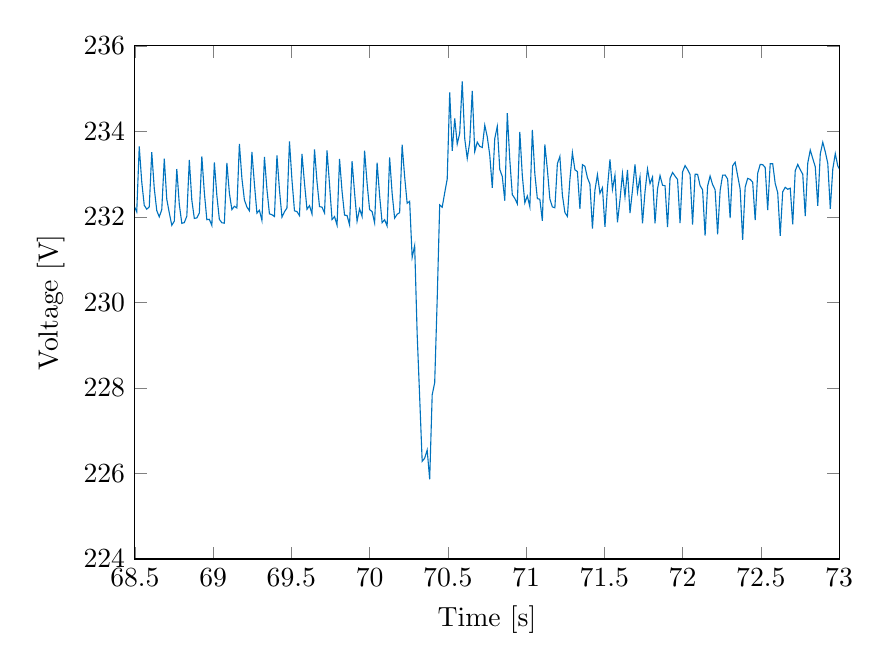
\begin{tikzpicture}

\begin{axis}[%
width=3.521in,
height=2.566in,
at={(0.758in,0.481in)},
scale only axis,
xmin=68.5,
xmax=73,
xlabel={Time [s]},
ymin=224,
ymax=236,
ylabel={Voltage [V]},
axis background/.style={fill=white}
]
\addplot [color=mycolor1,solid,forget plot]
  table[row sep=crcr]{%
68.496	232.251449569516\\
68.512	232.116248346484\\
68.528	233.64890076305\\
68.544	232.817435120229\\
68.56	232.269923036835\\
68.576	232.180268285985\\
68.592	232.232821803907\\
68.608	233.511499938504\\
68.624	232.664112503649\\
68.64	232.147245877425\\
68.656	232.000145361167\\
68.672	232.171771917135\\
68.688	233.359675912275\\
68.704	232.410735494188\\
68.72	232.094375321851\\
68.736	231.802547979314\\
68.752	231.899619719769\\
68.768	233.118656570701\\
68.784	232.291522758853\\
68.8	231.848666635778\\
68.816	231.866028285432\\
68.832	232.016802515841\\
68.848	233.329475099936\\
68.864	232.392386586747\\
68.88	231.963488845695\\
68.896	231.976358088346\\
68.912	232.088525089789\\
68.928	233.413210070936\\
68.944	232.569831812258\\
68.96	231.933734500629\\
68.976	231.942595585816\\
68.992	231.799574919604\\
69.008	233.275509754118\\
69.024	232.499853539223\\
69.04	231.94214887262\\
69.056	231.862138744768\\
69.072	231.853501090939\\
69.088	233.264494621304\\
69.104	232.553738631634\\
69.12	232.170578126516\\
69.136	232.24798440205\\
69.152	232.20806953032\\
69.168	233.70888655265\\
69.184	232.90285536249\\
69.2	232.397924917593\\
69.216	232.229201069961\\
69.232	232.141022686801\\
69.248	233.516567463417\\
69.264	232.769304097647\\
69.28	232.087818340009\\
69.296	232.154646498921\\
69.312	231.916663566561\\
69.328	233.404419681412\\
69.344	232.646428285034\\
69.36	232.070278841888\\
69.376	232.050233959554\\
69.392	232.008302098164\\
69.408	233.43973945943\\
69.424	232.634988087114\\
69.44	231.994070162002\\
69.456	232.118936247902\\
69.472	232.20973380642\\
69.488	233.764682120991\\
69.504	232.860295957641\\
69.52	232.141863935973\\
69.536	232.123827410259\\
69.552	232.030012072503\\
69.568	233.472663027735\\
69.584	232.787180540395\\
69.6	232.177124658009\\
69.616	232.261945125468\\
69.632	232.067984058275\\
69.648	233.580190321213\\
69.664	232.819259631877\\
69.68	232.239860434024\\
69.696	232.22736497349\\
69.712	232.091790564866\\
69.728	233.551880467081\\
69.744	232.758637754491\\
69.76	231.93658601535\\
69.776	232.007048897476\\
69.792	231.807541762637\\
69.808	233.352695966716\\
69.824	232.598915306936\\
69.84	232.040229644767\\
69.856	232.03147678331\\
69.872	231.814185187302\\
69.888	233.300024060635\\
69.904	232.563580181608\\
69.92	231.898440435307\\
69.936	232.187284998009\\
69.952	232.010504938726\\
69.968	233.550046886092\\
69.984	232.783378340032\\
70	232.169669817287\\
70.016	232.124472085576\\
70.032	231.862007222445\\
70.048	233.26619785203\\
70.064	232.502576213765\\
70.08	231.864389729332\\
70.096	231.933040748994\\
70.112	231.786971098717\\
70.128	233.388067890249\\
70.144	232.550971832024\\
70.16	231.971586256247\\
70.176	232.060278230971\\
70.192	232.098281647715\\
70.208	233.686849406811\\
70.224	232.939266674927\\
70.24	232.319253722182\\
70.256	232.363732118338\\
70.272	231.052725758443\\
70.288	231.328372653101\\
70.304	229.259754431011\\
70.32	227.784751038288\\
70.336	226.28486478479\\
70.352	226.356925362287\\
70.368	226.548439476999\\
70.384	225.864120663848\\
70.4	227.838874901422\\
70.416	228.122665437129\\
70.432	230.070294983649\\
70.448	232.279262348935\\
70.464	232.226236569789\\
70.48	232.562977263779\\
70.496	232.885104290305\\
70.512	234.912915461568\\
70.528	233.544008456963\\
70.544	234.302942230274\\
70.56	233.703073145207\\
70.576	233.956716467103\\
70.592	235.166499678207\\
70.608	233.828417969806\\
70.624	233.366437457811\\
70.64	233.748508481273\\
70.656	234.946354235433\\
70.672	233.5268004611\\
70.688	233.747655753545\\
70.704	233.650766154695\\
70.72	233.622130187609\\
70.736	234.14438942169\\
70.752	233.870781993417\\
70.768	233.443261203925\\
70.784	232.677160149025\\
70.8	233.834080616808\\
70.816	234.115885368237\\
70.832	233.109467044221\\
70.848	232.943595982628\\
70.864	232.378351183493\\
70.88	234.426809765027\\
70.896	233.330237546494\\
70.912	232.517375705827\\
70.928	232.433277201844\\
70.944	232.3053151428\\
70.96	233.985676469822\\
70.976	232.964033086596\\
70.992	232.328266747979\\
71.008	232.488591082381\\
71.024	232.237561173124\\
71.04	234.035578605595\\
71.056	233.006245118356\\
71.072	232.427967448264\\
71.088	232.411480576861\\
71.104	231.906205229016\\
71.12	233.691926419567\\
71.136	233.112715297968\\
71.152	232.420259178693\\
71.168	232.232833683056\\
71.184	232.213168363914\\
71.2	233.242117637983\\
71.216	233.413050973459\\
71.232	232.509843510641\\
71.248	232.103730175736\\
71.264	232.011593800413\\
71.28	232.873862407389\\
71.296	233.502280397913\\
71.312	233.101713809533\\
71.328	233.058715721681\\
71.344	232.185665093918\\
71.36	233.22179504934\\
71.376	233.183000508726\\
71.392	232.914980327856\\
71.408	232.768699022011\\
71.424	231.726194981156\\
71.44	232.623351243245\\
71.456	232.987747188635\\
71.472	232.550065998251\\
71.488	232.681556650507\\
71.504	231.765494360563\\
71.52	232.677137991314\\
71.536	233.344497956787\\
71.552	232.643590974936\\
71.568	232.976084471671\\
71.584	231.874407393658\\
71.6	232.397359717993\\
71.616	233.012505402917\\
71.632	232.469702165938\\
71.648	233.097730288341\\
71.664	232.086962718047\\
71.68	232.625717125542\\
71.696	233.225032909238\\
71.712	232.578377118452\\
71.728	232.931694318347\\
71.744	231.847870528491\\
71.76	232.588338461857\\
71.776	233.118576258087\\
71.792	232.776260080183\\
71.808	232.932596138131\\
71.824	231.850483809871\\
71.84	232.65430737604\\
71.856	232.964789271316\\
71.872	232.739939985592\\
71.888	232.727760396281\\
71.904	231.75899709317\\
71.92	232.900313494637\\
71.936	233.038003425124\\
71.952	232.953202651324\\
71.968	232.874070514084\\
71.984	231.85242909856\\
72	233.052528618872\\
72.016	233.199121197142\\
72.032	233.107627966594\\
72.048	232.989878579292\\
72.064	231.820997509231\\
72.08	232.99723764434\\
72.096	232.995013422302\\
72.112	232.731066394715\\
72.128	232.633071590528\\
72.144	231.560343716782\\
72.16	232.719514450675\\
72.176	232.954539851237\\
72.192	232.752864719806\\
72.208	232.634234996637\\
72.224	231.594253165812\\
72.24	232.616317893772\\
72.256	232.975630187318\\
72.272	232.978289128635\\
72.288	232.88340515495\\
72.304	231.972709539727\\
72.32	233.194203914211\\
72.336	233.278846366929\\
72.352	232.962757833268\\
72.368	232.650919924308\\
72.384	231.461561312247\\
72.4	232.693479050195\\
72.416	232.900231376653\\
72.432	232.876422128318\\
72.448	232.814832033489\\
72.464	231.923086283298\\
72.48	233.017461069544\\
72.496	233.226768742946\\
72.512	233.221343835813\\
72.528	233.154851966656\\
72.544	232.161370876316\\
72.56	233.242218288926\\
72.576	233.241088227942\\
72.592	232.782551987061\\
72.608	232.566069261898\\
72.624	231.557426985776\\
72.64	232.586667693532\\
72.656	232.690875521801\\
72.672	232.64557919328\\
72.688	232.669782435138\\
72.704	231.82799858649\\
72.72	233.079562012931\\
72.736	233.226746078392\\
72.752	233.102793936766\\
72.768	232.998336719037\\
72.784	232.019594405408\\
72.8	233.256925367217\\
72.816	233.562277673375\\
72.832	233.364482335795\\
72.848	233.171413821331\\
72.864	232.257525154906\\
72.88	233.471039555012\\
72.896	233.745193150055\\
72.912	233.520829146605\\
72.928	233.250933793244\\
72.944	232.187633628563\\
72.96	233.120881047595\\
72.976	233.476532248812\\
72.992	233.191304074376\\
73.008	233.079589031756\\
};
\end{axis}
\end{tikzpicture}% 
\caption{Voltage measured on all three phases with Hioki oscilloscope at 50 kHz sampling rate and RMS calculated, before and after a power step from 40 to 50 kW is performed on a genset located at DEIF. Data is then down sampled to 1 kHz and 16 samples is averaged to get a 62.5 Hz output.}
\label{fig:4050kwstepvoltage62.5hz}
\end{figure}

The 62.5 Hz sampling rate and the reduction in fluctuation shown between \figref{fig:4050kwstepvoltage50khz} and \figref{fig:4050kwstepvoltage62.5hz} is considered acceptable on the grounds, that the update interval to the governor is 25 Hz and an apparent change in Voltage is registered in the 1 kHz averaged 62.5 Hz measuring, when a change in load occurs. 
In order to be able to design a controller, modeling of the genset and inverter is needed. Along with the dynamics describing how changes in load affects voltage on the genset, the effects of frequency reference changes on the voltage output are also required. A block diagram, giving an overview of what needs to be modeled is shown in \figref{fig:gensetmodeling}.



\begin{figure}[H]
\centering
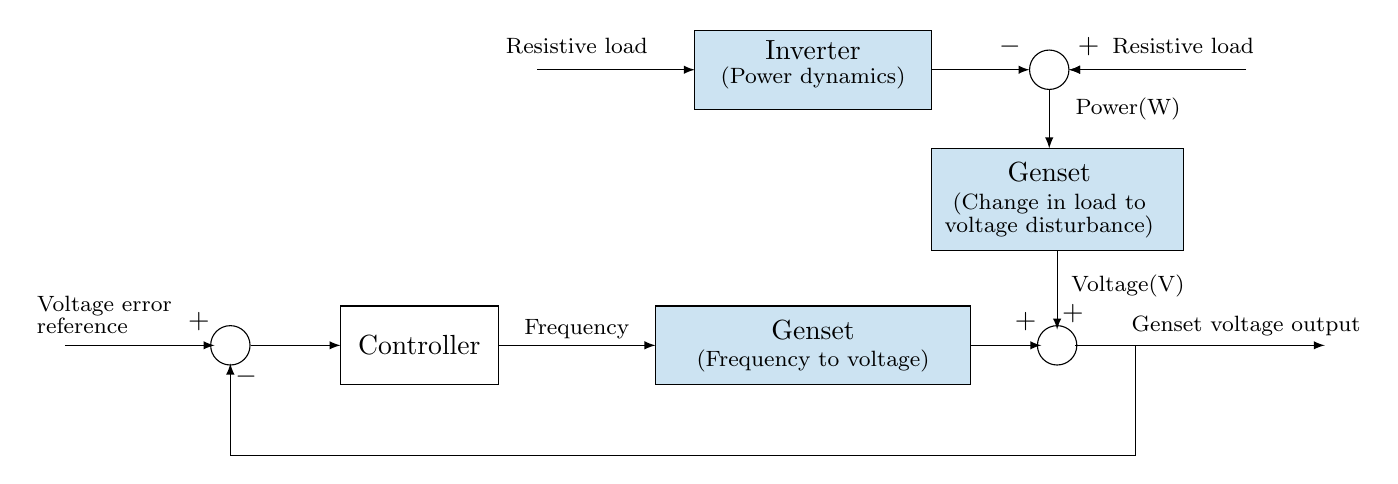
\begin{tikzpicture}
 \definecolor{mycolor1}{rgb}{0.00000,0.44700,0.74100} 
\draw  [fill=mycolor1!20](-5.5,2.5) rectangle (-1.5,1.5);
\draw [fill=mycolor1!20] (-2,4.5) rectangle (1.2,3.2);
\node at (-0.5,4.2) {\normalsize{Genset}};
\node at (-0.5,3.8) {\normalsize{\footnotesize{(Change in load to}}};
\node at (-0.5,3.5) {\normalsize{\footnotesize{voltage disturbance)}}};
\node at (-3.5,2.2) {\normalsize{Genset}};
\node at (-3.5,1.8) {\normalsize{\footnotesize{(Frequency to voltage)}}};

\draw [fill=mycolor1!20] (-5,6) rectangle (-2,5);
\draw [-latex] (-0.4,2) ellipse (0.25 and 0.25);
\draw [-latex](-1.5,2) -- (-0.6,2);
\draw [-latex](-0.4,3.2) -- (-0.4,2.2);
\draw [-latex] (-9.5,2.5) rectangle (-7.5,1.5);
\node at (-8.5,2) {Controller};
\draw [-latex](-7.5,2) -- (-5.5,2);

\node at (-0.2,2.4) {$+$};
\draw [-latex] (-10.9,2) ellipse (0.25 and 0.25);
\draw [-latex](-10.64,2) -- (-9.5,2);


\draw [-latex](-13,2) -- (-11.1,2);
\node at (-12.5,2.5) {\normalsize{\footnotesize{Voltage error}}};
\node at (-12.78,2.25) {\normalsize{\footnotesize{reference}}};
\draw [-latex](-0.17,2) -- (3,2);

\draw [-latex](0.6,2) -- (0.6,0.6) -- (-10.9,0.6) -- (-10.9,1.77);
\node at (-10.7,1.6) {$-$};
\node at (-11.3,2.3) {$+$};
\node at (-0.8,2.3) {$+$};
\node at (2,2.25) {\normalsize{\footnotesize{Genset voltage output}}};
\node at (-6.5,2.2) {\footnotesize{Frequency}};
\draw [-latex](2,5.5) -- (-0.25,5.5);
\node at (1.2,5.8) {\normalsize{\footnotesize{Resistive load}}};
\draw [-latex] (-0.5,5.5) ellipse (0.25 and 0.25);


\node at (-3.5,5.75) {\normalsize{Inverter}};
\node at (-3.5,5.4) {\normalsize{\footnotesize{(Power dynamics)}}};

\draw [-latex](2,5.5) -- (-0.25,5.5);
\draw [-latex](-2,5.5) -- (-0.75,5.5);
\draw [-latex](-0.5,5.25) -- (-0.5,4.5);
\draw [-latex](-7,5.5) -- (-5,5.5);

\node at (-6.5,5.8) {\normalsize{\footnotesize{Resistive load}}};
\node at (0.5,5) {\normalsize{\footnotesize{Power(W)}}};
\node at (0.5,2.75) {\normalsize{\footnotesize{Voltage(V)}}};

\node at (0,5.8) {$+$};
\node at (-1,5.8) {$-$};
\end{tikzpicture} 
%\includegraphics[width=0.6\textwidth]{rapport/billeder/genset_control_approach.png}
\caption{Block diagram showing combined inverter and genset with controller, where blocks in lightblue indicates systems to be modeled.}
\label{fig:gensetmodeling}
\end{figure}


%\begin{figure}[H]
%\centering
%\includegraphics[width=1\textwidth]{rapport/billeder/gensetmodeling.png}
%\caption{Block diagram showing combined inverter and genset with controller, where blocks in lightblue indicates systems to be modeled.}
%\label{fig:gensetmodeling}
%\end{figure}

For the sake of comparison between the simulation and measurements, genset systems for frequency to power and power to power models is added to the list of models to be derived. The derivation of the various models is to be described in the section to come. 



%The Voltage reference is given to the AVR as an RMS value of all three phases, which mean it needs to be calculated before it can be used by a controller. 


%On \figref{fig:4050kwstepfreq} and \figref{fig:4050kwstepvoltage50khz} frequency and Voltage is shown during a 40 to 50 kW step in load. 

% The RMS Voltage can be calculated by the following equation:

% \begin{equation} 
% \label{eq:Vrms}
% V_{RMS} = \sqrt{\frac{V_{1}^2+V_{2}^2+V_{3}^2}{3}}
% \end{equation}

% Where $V_1$, $V_2$ and $V_3$ is the individual phases.







%Due to the amount of noise at the output of the genset it will be difficult to control by  





%To correct the disturbance appearing when a change in load occurs as shown on \figref{fig:steps_model_comparison} a measurement on the output of the genset is necessary. This could be Voltage, current and electrical frequency, where Voltage and current could be used to calculate power output of the genset. The only known references given to the genset is frequency and Voltage

%\begin{figure}[H]
%\centering
%\includegraphics[width=0.75\textwidth]{rapport/billeder/blok}
%\caption{.}
%\label{fig:blok}
%\end{figure}

